\documentclass[10pt, landscape]{article}
\usepackage[scaled=0.92]{helvet}
\usepackage{calc}
\usepackage{multicol}
\usepackage[a4paper,margin=3mm,landscape]{geometry}
\usepackage{amsmath,amsthm,amsfonts,amssymb}
\usepackage{bm}
\usepackage{color,graphicx,overpic}
\usepackage{hyperref}
\usepackage{newtxtext} 
\usepackage{enumitem}
\usepackage[table]{xcolor}
\usepackage{mathtools}
\setlist{nosep}
% for including images
\graphicspath{ {./images/} }

\pdfinfo{
  /Title (ST2132.pdf)
  /Creator (TeX)
  /Producer (pdfTeX 1.40.0)
  /Author (Jovyn Tan)
  /Subject (ST2132)
/Keywords (ST2132, nus,cheatsheet,pdf)}

% Turn off header and footer
\pagestyle{empty}

% redefine section commands to use less space
\makeatletter
\renewcommand{\section}{\@startsection{section}{1}{0mm}%
  {-1ex plus -.5ex minus -.2ex}%
  {0.5ex plus .2ex}%x
{\normalfont\large\bfseries}}
\renewcommand{\subsection}{\@startsection{subsection}{2}{0mm}%
  {-1explus -.5ex minus -.2ex}%
  {0.5ex plus .2ex}%
{\normalfont\normalsize\bfseries}}
\renewcommand{\subsubsection}{\@startsection{subsubsection}{3}{0mm}%
  {-1ex plus -.5ex minus -.2ex}%
  {1ex plus .2ex}%
{\normalfont\small\bfseries}}%
\makeatother

\renewcommand{\familydefault}{\sfdefault}
\renewcommand\rmdefault{\sfdefault}
%  makes nested numbering (e.g. 1.1.1, 1.1.2, etc)
\renewcommand{\labelenumii}{\theenumii}
\renewcommand{\theenumii}{\theenumi.\arabic{enumii}.}
\renewcommand\labelitemii{•}
\renewcommand\labelitemiii{•}

\definecolor{mathblue}{cmyk}{1,.72,0,.38}
\everymath\expandafter{\the\everymath \color{mathblue}}

% Don't print section numbers
\setcounter{secnumdepth}{0}

\setlength{\parindent}{0pt}
\setlength{\parskip}{0pt plus 0.5ex}
%% adjust spacing for all itemize/enumerate
\setlength{\leftmargini}{0.5cm}
\setlength{\leftmarginii}{0.5cm}
\setlist[itemize,1]{leftmargin=2mm,labelindent=1mm,labelsep=1mm}
\setlist[itemize,2]{leftmargin=4mm,labelindent=1mm,labelsep=1mm}

\newcommand{\cov}{\mathop{\mathrm{cov}}}
\newcommand{\var}{\mathop{\mathrm{var}}}
\newcommand{\xbar}{\bar{x}}
\newcommand{\Xbar}{\bar{X}}
\newcommand{\seq}[2][n]{#2_1, \dots, #2_{#1}}

\DeclareRobustCommand{\svdots}{% s for `scaling'
  \vbox{%
    \baselineskip=0.33333\normalbaselineskip
    \lineskiplimit=0pt
    \hbox{.}\hbox{.}\hbox{.}%
    \kern-0.2\baselineskip
  }%
}

% adding my commands
% tightcenter
\newenvironment{tightcenter}{%
  \setlength\topsep{0pt}
  \setlength\parskip{0pt}
  \begin{center}
    }{%
  \end{center}
}

% boxed
\newenvironment{tightbox}{%
  \setlength\topsep{0pt}
  \setlength\parskip{0pt}
  \begin{center}
    \begin{tabular}{|@{\hspace{\dimexpr\fboxsep+0.5\arrayrulewidth}}c@{\hspace{\dimexpr\fboxsep+0.5\arrayrulewidth}}|}
      \hline
    }
    {%
    \\ \hline
    \end{tabular}
  \end{center}
}

% fixed width box
\newenvironment{fixedbox}[1][0.7]{
  \setlength\topsep{0pt}
  \setlength\parskip{0pt}
  \begin{center}
    \begin{tabular}{|>{\centering\arraybackslash}m{#1\linewidth}|}
    \hline
  }{
  \\ \hline
  \end{tabular}
  \end{center}
}

% definition of a new term
\usepackage{soul}
\definecolor{paleyellow}{RGB}{251,243,218}
\newcommand{\definition}[2][]{\sethlcolor{paleyellow}\hl{\textbf{#2}} #1  $\rightarrow$}
% inline definition
\newcommand{\ildefinition}[1]{\sethlcolor{paleyellow}\hl{\textbf{#1}}}

% important note (attention)
\newcommand{\attention}{{\color{red}\textbf{! }}}

% nice proof
\newenvironment{niceproof}[1][Proof]
{%
  \sbox0{\textit{#1}. }%
  \list{}{\labelwidth\wd0 \leftmargin\wd0 \labelsep 0pt }
\item[\usebox0]}
  {\endlist}


%  convenient absolute value symbol
\newcommand{\abs}[1]{\vert #1 \vert}

%  convenient floor and ceiling
\newcommand{\floor}[1]{\lfloor #1 \rfloor}
\newcommand{\ceil}[1]{\lceil #1 \rceil}

%  modulo with nicer spacing
\newcommand{\Mod}[1]{\ \mathrm{mod}\ #1}

%  convenient dx with nicer spacing
\newcommand{\dx}{\mathop{dx}}
\newcommand{\dy}{\mathop{dy}}



% -----------------------------------------------------------------------

\begin{document}
\raggedright
\footnotesize
\begin{multicols*}{4}
  % multicol parameters
  \setlength{\columnseprule}{0.25pt}

  \begin{center}
    \fbox{%
      \parbox{0.8\linewidth}{\centering \textcolor{black}{
          {\Large\textbf{ST2132}}
        \\ \normalsize{AY23/24 SEM 1}}
        \\ {\footnotesize \textcolor{gray}{github/jovyntls}}
      }%
    }
  \end{center}

  \section{01. PROBABILITY}

  \begin{itemize}
    \item \definition[of an event]{probability} the limiting relative frequency of its occurrence as the experiment is repeated many times
    \item the \textbf{realisation} $x$ is a constant, and $X$ is a generator
      \begin{itemize}
        \item running $r$ experiments gives us $r$ realisations $\seq[r]{x}$
      \end{itemize}
  \end{itemize}

  \subsection{Expectation}

  \begin{tightcenter}
    \begin{multicols*}{2}
      \textbf{discrete}: \\* (mass function) \\* \( {\displaystyle{ E(X) := \sum^n_{i=1}x_ip_i }} \) 

      \textbf{continuous}: \\* (density function) \\* \( {\displaystyle{ E(X) := \int^\infty_{-\infty} xf(x) \dx }} \) 
    \end{multicols*}
  \end{tightcenter}

  \subsubsection{expectation of a function $h(X)$}

  $ E\{h(X)\} = \begin{cases}
        \sum^n_{i=1} h(x_i)p_i &\text{$X$ is discrete} \\ 
        \int^\infty_{-\infty} h(x)f(x)\dx &\text{$X$ is continuous} \\ 
      \end{cases}$ 

  \subsection{Variance}

  \begin{tightcenter}
      \textbf{variance}, $\var(X) := E\{(X-\mu)^2\}$

    \textbf{standard deviation}, $SD(X) := \sqrt{\var(X)}$
  \end{tightcenter}

  \begin{itemize}
    \item $\var(X) = E(X^2) - E(X)^2$
    \item $E(X - \mu) = 0$
  \end{itemize}

  \subsection{Law of Large Numbers}

  mean and variance of $r$ realisations:  

  \begin{tightcenter}
    \( {\displaystyle{ \xbar := \frac{1}{r} \sum^r_{i=1} x_i }} \) 
    $\qquad$
    \( {\displaystyle{ v := \frac{1}{r}\sum^r_{i=1} (x_i - \xbar)^2 }} \) 
  \end{tightcenter}

  \textbf{LLN:} for a function $h$, as $r \to \infty$, 

  \begin{tightcenter}
    \( {\displaystyle{ \frac{1}{r} \sum^r_{i=1}h(x_i) \to E\{h(X)\}  }} \) 

    $\xbar \to E(X)$, $\quad v \to \var(X)$
  \end{tightcenter}

  \subsubsection{Monte Carlo approximation}

  simulate $\seq[r]{x}$ from $X$. by LLN, as $r \to \infty$, the approximation becomes exact

  \begin{tightcenter}
    \( {\displaystyle{ E\{h(X)\} \approx \frac{1}{r} \sum^r_{i=1} h(x_i) }} \) 
  \end{tightcenter}

  \subsection{Joint Distribution}

  (\textbf{discrete}) mass function:
  \begin{tightcenter}
    \( {\displaystyle{P( X = x_i, Y = y_j ) = p_{ij}}} \)  
  \end{tightcenter}

  (\textbf{continuous}) density function:
  \begin{tightcenter}
    \( {\displaystyle{f : \mathbb{R}^2  \to [0, \infty), \int^\infty_{-\infty} f(x, y) \dx \dy = 1}} \) 
  \end{tightcenter}

  (\textbf{expectation}) for $h : \mathbb{R}^2 \to \mathbb{R}$,
  \begin{tightcenter}
    \( {\displaystyle{ E\{ h(X,Y)\} = }} \) 
    \( {\displaystyle{ 
        \begin{cases}
          \sum^I_{i=1}\sum^J_{j=1} h(x_i, y_j) p_{ij} & X \text{ is discrete}
          \\ \int^\infty_{-\infty}\int^\infty_{-\infty} h(x, y) f(x, y) \dx \dy & Y \text{ is continuous}
        \end{cases}
    }} \) 
  \end{tightcenter}

  \subsection{Algebra of RV's}

  let $X, Y$ be RVs and $a, b, c$ be constants

  \begin{itemize}
    \item $Z = aX + bY + c$ is also an RV
      \begin{itemize}
        \item $z = ax + by + c$ is a realisation of $Z$
      \end{itemize}
    \item linearity of expectation: $E(Z) = aE(X) + bE(Y) + c$
    \item any theorem about a RV is true about a constant 
  \end{itemize}

  \subsection{Covariance}

  let $\mu_X = E(X)$, $\mu_Y=E(Y)$.

  \begin{tightcenter}
    \textbf{covariance}, $\cov(X,Y) = E\{ (X-\mu_X)(Y-\mu_Y) \}$
  \end{tightcenter}

  \begin{itemize}
    \item $\cov(X, Y) = E(XY) - \mu_X\mu_Y$
    \item $\cov(X, Y) = \cov(Y,X)$
    \item $\cov(X, X) = \var(X)$
    \item $\cov(W, aX+bY+c) = a\cov(W, X) + b\cov(W, Y)$
    \item $\var(aX + bY + c) = a^2 \var(X) + b^2 \var(Y) + 2ab\cov(X, Y)$
    \item $\var(\sum^N_{i=1}a_iX_i) = \sum^N_{i=1}a_i^2\var(X_i) + 2\sum_{1 \leq i < j \leq N} a_ia_j \cov(X_i,X_j)$
  \end{itemize}

  \subsection{joint $=$ marginal $\times$ conditional distributions}

  \begin{align*}
    f(x, y) &= f_X(x)f_Y(y \vert x) 
         \\ &= f_Y(y) f_X(x \vert y),  \quad x, y \in \mathbb{R}
  \end{align*}

  \begin{itemize}
    \item $f(x, y)$ is the \textit{joint density}
    \item $f_X(x), f_Y(y)$ are the \textit{marginal densities}
    \item $f_Y(\cdot \vert x)$ is the \textbf{conditional} density of $Y$ given $X=x$
    \item $f_X(\cdot \vert y)$ is the \textbf{conditional} density of $X$ given $Y=y$ 
    \item for discrete case, \textit{density} $\equiv$ \textit{probability}, $x \equiv x_i$, $y \equiv y_j$
  \end{itemize}


  \subsection{Independence}

  \begin{itemize}
    \item $X, Y$ are independent $\iff \forall x, y \in \mathbb{R}$, 

      \begin{enumerate}
        \item $f(x, y) = f_X(x)f_Y(y)$ 
        \item $f_Y(y\vert x) = f_Y(y)$
        \item $f_X(x\vert y) = f_Y(x)$
      \end{enumerate}

    \item $X, Y$ are independent  $\Rightarrow$
      \begin{itemize}
        \item $E(XY) = E(X)E(Y)$ 
        \item $\cov(X,Y) = 0$
      \end{itemize}
      (the converse does not hold)
  \end{itemize}

  \subsection{Conditional expectation}

  \subsubsection{discrete case}

  let $f_Y(\cdot \vert x_i)$ be the conditional pmf of $Y$ given $X = x_i$.

  \begin{tightcenter}
    \( {\displaystyle{ E[Y \vert x_i] := \sum^J_{j=1} y_j f_Y (y_j \vert x_i) }} \) 

    \( {\displaystyle{ \var[Y\vert x_i] := \sum^J_{j=1} (y_j - E[Y\vert x_i])^2 f_Y (y_j \vert x_i) }} \) 
  \end{tightcenter}

  $E[Y\vert x_i]$ is like $E(Y)$, with conditional distribution replacing marginal distribution  $f_Y(\cdot)$. 
  likewise, $\var[Y\vert x_i]$ like $\var(Y)$.

  \subsubsection{continuous case}

  \begin{tightcenter}
    \( {\displaystyle{ E[Y \vert x] := \int^\infty_{-\infty} y f_Y (y \vert x) \dy }} \) 
  \end{tightcenter}

  \begin{align*}
    \var[Y\vert x] &:= \int^\infty_{-\infty} (y - E[Y\vert x])^2 f_Y (y \vert x) \dy 
                \\ &= E(Y^2 \vert x) - \{E(Y \vert x)\}^2
  \end{align*}

  \subsection{Distributions}

  if $X$ is iid with expectation $\mu$, SD $\sigma$ and $S_n = \sum^n_{i=1}X_i$,

  \begin{itemize}
    \item  $ E(S_n) = n\mu$
    \item $SD(S_n) = \sqrt n \sigma $
    \item variance of sum = sum of variances
      $ \var(\sum^n_{i=1} X_i) = \sum^n_{i=1} \var(x_i) $ 
  \end{itemize}

  \subsubsection{bernoulli}

  $X \sim Bernoulli(p) \quad \Rightarrow$ coin flip with probability $p$

  \begin{tightcenter}
    $E(X_i) = p \qquad \var(X_i) = p(1-p)$
    $E(S_n) = np \qquad \var(S_n) = np(1-p)$
  \end{tightcenter}

  \subsubsection{binomial}

  $X \sim Bin(n, p) \quad \Rightarrow$ 
  $X_i \mathop{\sim}\limits^{i.i.d.} Bernoulli(p)$

  \begin{tightcenter}
    $E(X) = np, \quad \var(X) = np(1-p)$

    \( {\displaystyle{ E(X) = \sum^n_{k=1} k \binom{n}{k} p^k (1-p)^{n-k} }} \)  

    $\cov(X,n-X) = -\var(X)$
  \end{tightcenter}

  \subsubsection{multinomial}

  $X \sim Multinomial(n, \mathbf{p})$ 

  \begin{itemize}
    \item for $k$ outcomes $\seq[k]{E}$, $\; Pr(E_i) = p_i$.
      For some $1 \leq i \leq k$, $E_i$ occurs $X_i$ times in $n$ runs.
  \end{itemize}

  $(\seq[k]{X})$ has the \textbf{multinomial distribution:}

  \begin{tightcenter}
    \( {\displaystyle{ Pr(X_1 = x_1, \dots, X_k = x_k) = \binom{n}{\seq[k]{x}} \Pi^k_{i=1} p_i^{x_i} }} \)   
  \end{tightcenter}

  \begin{itemize}
    \item where $\binom{n}{\seq[k]{x}} = \frac{n!}{x_1! x_2! \dots x_k!}$
      \begin{itemize}
        \item combinatorially, \# of arrangements of $\seq[k]{x}$
        \item $\sum^n_{i=1}x_i = n, \quad x_i \ge 0$
      \end{itemize}
  \end{itemize}

  \begin{tightcenter}
    $E(X) = \left[\begin{smallmatrix}np_1 \\ np_2 \\ \svdots \\ np_k\end{smallmatrix}\right]$,  
    $\quad \var(X_i) = np_i (1-p_i)$

    $\var(X) =$ \textit{covariance matrix} $M$ with $m_{ij} = \begin{cases}
      \var(X_i) & \text{if }i=j
      \\ \cov(X_i, X_j) & \text{if }i \neq j
    \end{cases} $
  \end{tightcenter}

  \begin{itemize}
    \item $\cov(X_i, X_j) < 0$
    \item $X_i \sim Bin(n, p_i)$
    \item $X_i + X_j \sim Bin(n, p_i + p_j)$
  \end{itemize}


  \section{02. PROBABILITY (2)}

  \subsection{Mean Square Error (MSE)}

  $$MSE = E\{ (Y-c)^2 \}$$

  \begin{itemize}
    \item predicting Y:
      \\* $MSE = \var(Y) + \{ E(Y) - c\}^2$
      \begin{itemize}
        \item $\min MSE=\var(Y)$ when $c = E(Y)$
      \end{itemize}
    \item $Y$ and $X$ are correlated: 
      \\* $MSE = \var[Y \vert x] + \{ E[Y\vert x] - c \}^2$
      \\* $MSE = E[(Y-c)^2 \vert x] = E[\{ Y - E(Y) \}^2 \vert x]$
      \begin{itemize}
        \item $\min MSE = \var(Y \vert x)$ when $c = E[Y \vert x]$
        \item if $c = E(Y)$ instead of $E(Y \vert x)$ $\Rightarrow$ the MSE increases by $( E(Y \vert x) - E(Y) )^2$
      \end{itemize}
  \end{itemize}

  \subsubsection{mean MSE}

  $$\frac{1}{n} \sum^n_{i=1}\var[Y \vert x_i] \approx E\{ \var[Y \vert X] \}$$

  \subsubsection{random conditional expectations}

  let $X, Y$ be r.v.s.
  \begin{itemize}
    \item $E[Y \vert X]$ is a r.v. which takes value $E[Y \vert x]$ with probability/density $f_X(x)$
    \item $\var[Y \vert X]$ is a r.v. which takes value $\var[Y \vert x]$ with probability/density $f_X(x)$ 
  \end{itemize}

  \begin{tightcenter}
    $E(E[X_2 \vert X_1]) = E(X_2)$

    $\var(E[X_2 \vert X_1]) + E(\var[X_2 \vert X_1]) = \var(X_2)$
  \end{tightcenter}

  \subsection{CDF (cumulative distribution function)}

  for r.v. $X$, let $F(x) = P(X \leq x)$

  \begin{itemize}
    \item domain: $\mathbb{R}$; $\;$ codomain: $[0,1]$
  \end{itemize}

  \begin{tightcenter}
    $F(x) = \int^x_{-\infty} f(x) \dx$
  \end{tightcenter}

  \subsection{Standard Normal Distribution}

  \begin{tightcenter}
    $Z \sim N(0, 1)$ has density function \\* 
    \( {\displaystyle{ \phi(z) = \frac{1}{\sqrt{2\pi}} \exp \{ -\frac{z^2}{2} \}, \quad -\infty < z < \infty }} \) 
  \end{tightcenter}

  $$E(Z) = 0, \quad \var(Z) = 1$$

  \begin{tightcenter}
    \textbf{CDF}, $\Phi(x) = P(Z \leq x) = \int^x_{-\infty} \phi(z) \mathop{dz}$
  \end{tightcenter}

  \begin{itemize}
    \item  $E(Z) = \int^\infty_{-\infty} z\phi(z) \mathop{dz} = 0$
      \begin{itemize}
        \item  $E(Z^2) = \int^\infty_{-\infty} z^2\phi(z) \mathop{dz} = 1$
          \item $E(Z^{2k+1}) = 0 \quad \forall k \in \mathbb{Z}_{\ge 0}$
      \end{itemize}
  \end{itemize}

  \subsubsection{general normal distribution}

  let  $X \sim N(\mu, \sigma^2)$ and $Y \sim N(\nu, \tau^2)$

  \begin{tightcenter}
    \textbf{standardisation:} $\frac{X - \mu}{\sigma} \sim N(0, 1)$
  \end{tightcenter}

  \begin{itemize}
    \item summations: 
      \begin{itemize}
        \item for constants $a, b \neq 0$, 
          \\* $\quad \; a + bX \sim N(a+b\mu, \; b^2\sigma^2)$
        \item $X + Y \sim N(\mu + \nu, \; \sigma^2 + \tau^2 + 2\cov(X,Y))$
          \begin{itemize}
            \item $\cov(X, Y) = 0$, $\quad \Rightarrow \quad$ $X \perp Y$
            \item $X \perp Y$ $\quad \Rightarrow \quad$ $X + Y \sim N(\mu + \nu, \; \sigma^2 + \tau^2)$
          \end{itemize}
      \end{itemize}

    \item for $W = a + bX$, 
      \begin{itemize}
        \item density,  $f_W(w) = \frac{d}{dw} F_W(w)$
        \item CDF, $\;\;\; F_W(w) = P(X \leq \frac{w-a}{b}) = \Phi(\frac{w-a}{b})$
      \end{itemize}
  \end{itemize}

  \subsection{Central Limit Theorem}

  let $\seq{X}$ be iid rv's with expectation $\mu$ and SD $\sigma$, with $ S_n = \sum^n_{i=1} X_i $

  \begin{tightcenter}
    \textbf{CLT} 
    \\* as $n \to \infty$, the distribution of the standardised $S_n = \frac{S_n - n\mu}{\sqrt{n}\sigma}$ converges to $N(0,1)$
  \end{tightcenter}

  \begin{itemize}
    \item $E(S_n) = n\mu$, $\; \var(S_n) = n\sigma^2$
    \item for large $n$, approximately $S_n \sim N(n\mu, n\sigma^2)$
  \end{itemize}

  \subsubsection{bernoulli}

  let $X_i \sim Bernoulli(p)$. then $S_n \sim Binom(n, p)$
  \begin{itemize}
    \item for large $n$, $S_n \sim N(np, np(1-p))$
    \item CLT: standardised $\frac{S_n - np}{\sqrt{n}\sqrt{p(1-p)}} \to N(0,1)$ as $n \to \infty$
  \end{itemize}

  \subsection{Distributions}

  \subsubsection{chi-square ($\chi^2$)}

  let $Z \sim N(0,1)$. 
  $\quad\Rightarrow$ then $Z^2 \sim \chi^2_1$

  \begin{itemize}
    \item $Z^2$ has $\chi^2$ distribution with 1 degree of freedom
    \item degrees of freedom = number of RVs in the sum
  \end{itemize}

  \begin{tightcenter}
    $E(Z^2) = 1, \quad E(Z^4) = 3$
    \\* $\var(Z^2) = E(Z^4) - \{ E(Z^2) \}^2 = 2$
  \end{tightcenter}

  let $\seq{V}$ be iid $\chi^2_1$ RVs and $V = \sum^n_{i=1}V_i$. then 
  \begin{tightcenter}
    $V \sim \chi^2_n$

    $E(V) = n \quad \var(V) = 2n$
  \end{tightcenter}

  \subsubsection{gamma}

  \begin{tightcenter}
    let $\alpha, \lambda > 0$. The $Gamma(\alpha, \lambda)$ density is 
    \\* \( {\displaystyle{ \frac{\lambda^\alpha}{\Gamma(\alpha)} x^{\alpha-1} e^{-\lambda x}, \quad x > 0 }} \) 
    \\* where $\Gamma(\alpha)$ is a number that makes density integrate to 1
  \end{tightcenter}

  \begin{itemize}
    \item $\chi^2_n$ RV $\sim Gamma(\frac{n}{2}, \frac{1}{2})$
      \begin{itemize}
        \item $\chi^2_n$ is a special case of Gamma!
        \item density of $\chi_1^2$ RV $= \frac{1}{\sqrt{2\pi}} v^{-1/2} e^{-v/2}, \quad v > 0$
          \\* $\qquad\qquad\qquad\quad\;\; = Gamma(\frac{1}{2}, \frac{1}{2})$
      \end{itemize}
    \item if $X_1 \sim Gamma(\alpha_1, \lambda)$ and $X_2 \sim Gamma(\alpha_2, \lambda)$ are independent, then $X_1 + X_2 \sim Gamma(\alpha_1 + \alpha_2, \lambda)$
  \end{itemize}

  \subsubsection{t distribution}

  let $Z \sim N(0, 1)$ and $V \sim \chi^2_n$ be independent. 

  \begin{tightcenter}
    $\frac{Z}{\sqrt{V/n}} \sim t_n $
    \\* has a $t$ distribution with $n$ degrees of freedom.
  \end{tightcenter}

  \begin{itemize}
    \item $t$ distribution is symmetric around 0
    \item $t_n \to Z \;$ as $\; n \to \infty$ (because $\frac{V}{n} \to 1$)
  \end{itemize}

  \subsubsection{\textit{F} distribution}

  let $V \sim \chi^2_m$ and $W \sim \chi^2_n$ be independent. 

  \begin{tightcenter}
    $\frac{V/m}{W/n} \sim F_{m,n}$ 
    \\* has an $F$ distribution with $(m,n)$ degrees of freedom.
  \end{tightcenter}

  \begin{itemize}
    \item even if $m=n$, still two RVs $V,W$ as they are independent
    \item for $T \sim t_n$, $T^2 = \frac{Z^2}{V/n} \sim F_{1,n}$
  \end{itemize}

  \subsection{IID Random Variables}

  let $\seq{X}$ be iid RVs with mean $\bar{X}$. 

  \begin{tightcenter}
    \textbf{sample variance}, \( {\displaystyle{ S^2 = \frac{1}{n-1} \sum^n_{i=1} (X_i - \bar{X})^2 }} \) 

    $S$ is an estimate of $\sigma$
  \end{tightcenter}

  let $\seq{X}$ be iid $N(\mu, \sigma^2)$. $\bar{X} = \frac{1}{n} \sum^n_{i=1} X_i$. 
  \begin{tightcenter}
    $\bar{X} \sim N(\mu, \frac{\sigma^2}{n})$

    $E(\bar{X}) = \mu$, $\quad\var(\bar{X}) = \frac{\sigma^2}{n}$
  \end{tightcenter}

  more distributions:
  \begin{tightcenter}
    $\frac{\bar{X} - \mu}{\sigma/\sqrt{n}} \sim N(0,1)$

    $\frac{(n-1)S^2}{\sigma^2} \sim \chi^2_{n-1}$

    $\frac{\bar{X} - \mu}{S/\sqrt{n}} \sim t_{n-1}$
  \end{tightcenter}

  \begin{itemize}
    \item $\bar{X}$ and $S^2$ are independent
  \end{itemize}

  \subsection{Multivariate Normal Distribution}

  let $\bm{\mu}$ be a $k \times 1$ vector and $\bm{\Sigma}$ be a \textit{positive-definite} symmetric $k \times k$ matrix.

  \begin{tightcenter}
    the random vector $\bm{X} = (\seq[k]{X})'$ has a multivariate normal distribution $N(\bm{\mu}, \bm{\Sigma})$ if its density function is 

    \( {\displaystyle{ \frac{1}{(2\pi)^{k/2} \sqrt{det\bm{\Sigma}}} \exp \left(-\frac{(\bm{x} - \bm{\mu})' \bm{\Sigma}^{-1}(\bm{x} - \bm{\mu})}{2}\right) }} \) 
  \end{tightcenter}

  \begin{itemize}
    \item $E(\bm{X}) = \bm{\mu}, \quad \var(\bm{X}) = \bm{\Sigma}$
    \item for any non-zero $k \times 1 $ vector $\bm{a}$, 
      \begin{tightcenter}
        $\bm{a'X} \sim N(\bm{a'\mu}, \bm{a'\Sigma a})$
      \end{tightcenter}
      \begin{itemize}
        \item $\bm{a}'\bm{\Sigma a} > 0$ because $\bm{\Sigma}$ is positive-definite
        \item the product $\bm{a'X}$ is a scalar (same for $\bm{a'\mu}, \bm{a'\Sigma a}$)
      \end{itemize}
    \item two multinomial normal random vectors $\bm{X}_1$ and $\bm{X}_2$, sizes $h$ and $k$, are independent if $\cov (\bm{X}_1, \bm{X}_2) = \bm{0}_{h \times k}$
      \begin{itemize}
        \item $(X_1-\Xbar, \dots, X_n - \Xbar)$ has a multivariate normal distribution; $\;$
          the covariance between $\Xbar$ and $(X_1-\Xbar, \dots, X_n - \Xbar)$ is $0$, thus they are independent
      \end{itemize}
  \end{itemize}

  \section{03. POINT ESTIMATION}

  for a variable $v$ in population $N$, 
  \begin{tightcenter}
    \( {\displaystyle{ 
        \mu = \frac{1}{N} \sum^N_{i=1} v_i
        \quad \quad 
        \sigma^2 = \frac{1}{N} \sum^N_{i=1} (v_i - \mu)^2
    }} \) 
  \end{tightcenter}

  \begin{itemize}
    \item $\mu, \;\sigma^2$ are \ildefinition{parameters} (unknown constants)
    \item a \textbf{simple random sample} is used to estimate parameters: individuals drawn from the population at random without replacement
  \end{itemize}

  \subsubsection{binary variable}

  for variable $v$ with proportion $p$ in the population,

  \begin{tightcenter}
    $\mu = p, \qquad \sigma^2 = p(1-p)$
  \end{tightcenter}

  \subsubsection{single random draw}

  for variable $v$ (population of size $N$, mean $\mu$, variance $\sigma^2$),
  let $X$ be the chosen $v$-value.

  \begin{tightcenter}
    $E(X) = \mu$, $\qquad \var(X) = \sigma^2$
  \end{tightcenter}

  \subsubsection{draws with replacement}

  let $\seq{X}$ be random draws with replacement from a population of mean $\mu$ and variance $\sigma^2$.

  \begin{tightcenter}
    random sample mean, \( {\displaystyle{ \Xbar = \frac{1}{n}\sum^n_{i=1}X_i }} \) 

    $\seq{X}$ are iid with $E(X_i) = \mu$, $\var(X_i) = \sigma^2$

    $E(\Xbar) = \mu$, $\var(\Xbar) = \frac{\sigma^2}{n}$
  \end{tightcenter}

  let $\seq{x}$ be realisations of $n$ random draws with replacement from the population.

  \begin{tightcenter}
    sample mean, \( {\displaystyle{ \xbar = \frac{1}{n} \sum^n_{i=1} x_i }} \) 

  \end{tightcenter}

  \begin{itemize}
    \item as $n \to \infty$, $\xbar \to \mu$  (LLN)
    \item sample distribution, $x_i$ has the same distribution as $X_i$ and the population distribution 
  \end{itemize}

  \subsubsection{representativeness}

  \begin{itemize}
    \item $\seq{X}$ is \textbf{representative} of the population
      \begin{itemize}
        \item as $n$ gets larger, $\Xbar$ gets closer to $\mu$
      \end{itemize}
    \item $\seq{x}$ are \textit{likely} representative of the population
  \end{itemize}

  \subsection{estimating mean}

  given data $\seq{x}$, 

  \begin{itemize}
    \item sample mean, $ \xbar = \frac{1}{n} \sum^n_{i=1} x_i $ is an  \ildefinition{estimate} of $\mu$
    \item the error in $\xbar$ is $\mu - \xbar$; $\quad$ it cannot be estimated
    \item $\xbar$ is a realisation of the \textbf{estimator} $\Xbar$
      \begin{itemize}
        \item this realisation is used to estimate $\mu$
      \end{itemize}
  \end{itemize}

  \subsubsection{standard error}

  the size of error in estimate $\xbar$ is roughly \( {\displaystyle{ SD(\Xbar) = \frac{\sigma}{\sqrt{n}} }} \)   

  the \textbf{standard error} (SE) in $\xbar$ is $\frac{\sigma}{\sqrt{n}}$

  \begin{itemize}
    \item SE is a constant by definition: $SE = SD(\Xbar) = \frac{\sigma}{\sqrt{n}}$
  \end{itemize}

  \subsubsection{estimating $\sigma$}

  intuitive estimate of $\sigma^2$, $\hat{\sigma}^2 = \frac{1}{n} \sum^n_{i=1} (x_i-\xbar)^2 $

  \begin{tightcenter}
    sample variance, \( {\displaystyle{ s^2 = \frac{1}{n-1} \sum^n_{i=1} (x_i-\xbar)^2 }} \) 

    $E(s^2) = \sigma^2$
  \end{tightcenter}

  \subsection{Point estimation of mean}

  a population (size $N$) has unknown mean $\mu$, variance $\sigma^2$.

  for random draws (without replacement) $\seq{x}$: 

  $\xbar$ is a realisation of $\Xbar$, with $E(\Xbar) = \mu$, $\var(\Xbar) = \frac{\sigma^2}{n}$

  \begin{itemize}
    \item $\mu$ is estimated as $\xbar = \frac{1}{n} \sum^n_{i=1} x_i$ 
    \item error in $\xbar$ is measured by the SE: $\frac{\sigma}{\sqrt n} = SD(\Xbar)$
    \item SE is estimated as $\frac{s}{\sqrt n}$
  \end{itemize}

  $\Rightarrow$ $\mu$ is around $\xbar$, give or take $\frac{s}{\sqrt n}$ 

  \subsubsection{unbiased estimation}

  \begin{itemize}
    \item since $E(\Xbar) = \mu$, $\Xbar$ is an \textbf{unbiased} estimator of $\mu$. $\xbar$ is an unbiased estimate.
    \item $S^2$ is unbiased for $\sigma^2$: $E(S^2) = \sigma^2$
    \item $S$ is \textit{not} unbiased for $\sigma$: $E(S) < \sigma$
  \end{itemize}

  \subsection{Simple random sampling (SRS)}

  $n$ random draws \textit{without replacement} from a population of mean $\mu$ and variance $\sigma^2$. 

  \begin{itemize}
    \item for $i = 1, \dots, n$, $E(X_i) = \mu$ and $\var(X_i) = \sigma^2$ 
    \item for $i \neq j$, $\cov(X_i, X_j) = -\frac{\sigma^2}{N-1}$
  \end{itemize}

  \begin{itemize}
    \item if $n/N$ is relatively large, 
      \begin{itemize}
        \item multiply SE by correction factor $\sqrt \frac{N-n}{N-1}$
        \item standard error = $\frac{N-n}{N-1}$ 
      \end{itemize}
      $$E(\Xbar) = \mu, \quad \var(\Xbar) = \frac{N-n}{N-1}\frac{\sigma^2}{n}$$
    \item if $n << N$, then SRS is like sampling \textit{with replacement}
      (treat the data as if they come from IID RVs $\seq{X}$)
      $$E(\Xbar) = \mu, \quad \var(\Xbar) = \frac{\sigma^2}{n}$$
  \end{itemize}

  \subsubsection{estimating proportion $p$}

  \begin{itemize}
    \item in a 0-1 population, $\mu = p$, $\quad \sigma^2 = p(1-p)$
      \begin{itemize}
        \item $p$ is estimated as $\xbar$ (sample proportion of 1's)
      \end{itemize}
    \item $SE = \frac{\sqrt{p(1-p)}}{\sqrt n} = SD(\hat p)$
      \begin{itemize}
        \item estimated by replacing $p$ with $\xbar$
      \end{itemize}
    \item unbiased estimator $\hat p$
      \begin{itemize}
        \item $E(\hat p) = p, \quad \var(\hat p) = \frac{p(1-p)}{n}, \quad SD(\hat p) = SE$
      \end{itemize}
    \item the estimate of $\sigma$ is $\hat{\sigma}$, not $s$
    \item e.g. if a SRS of size 100 has 78 white balls, $p \approx 0.78 \pm \frac{\sqrt{0.78 \times 0.22}}{\sqrt {100}}$
  \end{itemize}

  \subsection{Gauss Model}

  Let $x_i$ be a realisation of $X_i$. $\seq[100]{X}$ are random draws with replacement from an imaginary population with mean $w$ and variance $\sigma^2$.
  $w$ and $\sigma^2$ are parameters (unknown constants).

  \begin{itemize}
    \item $E(X_i) = w, \quad \var{X_i} = \sigma^2$ (since $X_i$ is just 1 draw) 
    \item $E(\Xbar) = w, \quad \var{\Xbar} = \frac{\sigma^2}{100}$  
  \end{itemize}

  \section{04. ESTIMATION (SE, bias, MSE)}

  let $\seq{x}$ be from random draws $\seq{X}$ with replacement from a population of mean $\mu$ and variance $\sigma^2$.

  \begin{tightcenter}
    sample mean $\xbar$ is an \textit{unbiased estimate} of $\mu$

    $\xbar = \frac{1}{n} \sum^n_{i=1} x_i$

    SE = $\frac{\sigma}{\sqrt n} \approx \frac{s}{\sqrt n}$ tells us roughly how far $\xbar$ is from $\mu$

    sample variance, $s^2 = \frac{1}{n-1} \sum^n_{i=1} (x_i-\xbar)^2$
  \end{tightcenter}

  \subsection{MSE and bias}

  suppose measurements were from a population with mean $w + b$ where
  $b$ is a constant:
  $\quad x_i = w + b + \epsilon_i$
  \begin{itemize}
    \item $E(\Xbar) = w + b$
    \item $SD(\Xbar) = \frac{\sigma}{\sqrt n}$
      \begin{itemize}
        \item $SE = \frac{\sigma}{\sqrt n}$ measures how far $\xbar$ is from $w+b$, not $w$
      \end{itemize}
    \item if $b\neq 0$, then $\xbar$ is a biased estimate for $w$
  \end{itemize}

  \begin{tightcenter}
    $MSE = E\{(\Xbar - w)^2\} = \frac{\sigma^2}{n} + b^2$

    $MSE = SE^2 + bias^2$
  \end{tightcenter}

  as $n \to \infty, \; MSE \to b^2$

  \subsubsection{conclusion}

  \begin{tightcenter}
    let $\theta$ be a parameter (constant) and $\hat \theta$ be an estimator (RV).

    $SE = SD(\hat\theta)$, bias = $E(\hat\theta) - \theta$, 

    MSE = $E\{(\hat\theta - \theta)^2 = SE^2 + bias^2\}$
  \end{tightcenter}

  \section{05. INTERVAL ESTIMATION}

  let $\seq{x}$ be realisations of IID RVs $\seq{X}$ with unknown $\mu = E(X_i)$ and $\sigma^2 = \var(X_i)$. 

  sample mean, $\xbar = \frac{1}{n} \sum^n_{i=1}x_i$

  sample variance, $s^2 = \frac{1}{n-1} \sum^n_{i=1}(x_i-\xbar)^2$

  standard error, $SE = \frac{s}{\sqrt n}$

  \begin{tightcenter}
    \textbf{point estimation:} $\mu \approx \xbar$, give or take $\frac{s}{\sqrt n}$

    \textbf{interval estimation:} interval contains $\mu$ with some confidence level
  \end{tightcenter}

  interval estimation works well if
  \begin{itemize}
    \item $X_i$ has a normal distribution, for any $n > 1$ 
    \item $X_i$ has any other distribution but $n$ is large
  \end{itemize}

  \subsection{normal ''upper-tail quantile'' $z_p$}

  \begin{tightcenter}
    let $Z \sim N(0,1)$. for $0 < p < 1$, let $z_p$ be such that 

    $p=\Pr(Z > z_p)$
  \end{tightcenter}

  \begin{itemize}
    \item e.g. $z_{0.5} = 0$
    \item $z_p = (1-p)$-quantile of $Z$ 
    \item for $0<p<0.5$, $\Pr(-z_p \leq Z \leq z_p) = 1-2p$
  \end{itemize}

  \subsubsection{(case 1) normal distribution with known $\sigma^2$}

  assume $\seq{X}$ are IID $\sim N(0,1)$ with known $\sigma^2$.

  for $0<\alpha<1$, $\;\Pr(-z_{\frac{\alpha}{2}} \leq Z \leq z_{\frac{\alpha}{2}}) = 1-\alpha$

  \begin{tightcenter}
    \textbf{confidence interval for $\mu$:}
    the random interval 

    \( {\displaystyle{ \left( \Xbar-z_{\frac{\alpha}{2}}\frac{\sigma}{\sqrt n}, \Xbar+z_{\frac{\alpha}{2}}\frac{\sigma}{\sqrt n} \right) }} \) 

    contains $\mu$ with probability $1-\alpha$,

    and produces the realisation 
    $ \left( \xbar-z_{\frac{\alpha}{2}}\frac{\sigma}{\sqrt n}, \xbar+z_{\frac{\alpha}{2}}\frac{\sigma}{\sqrt n} \right) $
  \end{tightcenter}

  \begin{itemize}
    \item $1-\alpha$ is the \textbf{confidence level}
    \item \textit{Proof.} since $\frac{\Xbar - \mu}{\sigma / \sqrt n} \sim N(0,1)$,
      \begin{itemize}
        \item $\quad \Pr(-z_{\frac{\alpha}{2}} \leq \frac{\Xbar - \mu}{\sigma / \sqrt n} \leq z_{\frac{\alpha}{2}}) = 1 - \alpha$
          % \item $\quad \Pr(\mu-z_{\frac{\alpha}{2}}\frac{\sigma}{\sqrt n} \leq \Xbar \leq \mu + z_{\frac{\alpha}{2}}\frac{\sigma}{\sqrt n}) = 1 - \alpha$

        \item $\quad \Pr(\Xbar-z_{\frac{\alpha}{2}}\frac{\sigma}{\sqrt n} \leq \mu \leq \Xbar + z_{\frac{\alpha}{2}}\frac{\sigma}{\sqrt n}) = 1 - \alpha$
      \end{itemize}
  \end{itemize}

  \subsubsection{(case 2) normal distribution with unknown $\sigma^2$}

  assume $\seq{X}$ are IID $\sim N(\mu, \sigma^2)$ with unknown $\sigma^2$.

  replace $\sigma$ with $S$:

  \begin{tightcenter}
    for $0 < p < 1$, let $t_{p,n}$ be such that 

    $\Pr(t_n > t_{p,n}) = p$
  \end{tightcenter}

  \begin{itemize}
    \item $t_{p,n}$ is the \textit{upper} $p$ quartile of the $t$ distribution with $n$ degrees of freedom
      \begin{itemize}
        \item e.g. $t_{0.1,5} = 1.48$ (using $qt(0.9,5)$)
      \end{itemize}
    \item as $n \to \infty, \;\; t_{n,p} \to z_p$
    \item $\frac{\Xbar - \mu}{S/\sqrt n} \sim t_{n-1}$
    \item $\Pr( \Xbar - t_{\frac{\alpha}{2}, n-1} \frac{S}{\sqrt n} \leq \mu \leq \Xbar + t_{\frac{\alpha}{2}, n-1} \frac{S}{\sqrt n})$
  \end{itemize}

  \begin{tightcenter}
    the random interval

    $\left(\Xbar - t_{\frac{\alpha}{2}, n-1} \frac{S}{\sqrt n},  \Xbar + t_{\frac{\alpha}{2}, n-1} \frac{S}{\sqrt n}\right)$

    contains $\mu$ with probability $1-\alpha$.
  \end{tightcenter}

  \begin{itemize}
    \item data $\seq{x}$ give realisations $\xbar$ of $\Xbar$ and $s$ of $S$, thus the random interval gives a $(1-\alpha)$-CI for $\mu$: 
      $\left(\xbar - t_{\frac{\alpha}{2}, n-1} \frac{s}{\sqrt n},  \xbar + t_{\frac{\alpha}{2}, n-1} \frac{s}{\sqrt n}\right)$
  \end{itemize}

  \subsubsection{(case 3) general distribution with unknown $\sigma^2$}

  IID $\seq{X}$ with $E(X_i) =\mu$, $\var(X_i) = \sigma^2$ unknown

  \begin{itemize}
    \item for large $n$, approximately $\frac{S_n - n\mu}{\sqrt n \sigma} \sim N(0,1)$
    \item since $\frac{S_n - n\mu}{\sqrt n \sigma} \sim N(0,1) =  \frac{\Xbar - \mu}{\sigma / \sqrt n}$ and $S \approx \sigma$ for large $n$,
      \begin{itemize}
        \item $\quad \Pr(-z_{\frac{\alpha}{2}} \leq \frac{\Xbar - \mu}{\sigma / \sqrt n} \leq z_{\frac{\alpha}{2}}) \approx 1 - \alpha$
        \item $\quad \Pr(\Xbar-z_{\frac{\alpha}{2}}\frac{\sigma}{\sqrt n} \leq \mu \leq \Xbar + z_{\frac{\alpha}{2}}\frac{\sigma}{\sqrt n}) \approx 1 - \alpha$
      \end{itemize}
  \end{itemize}

  \begin{tightcenter}
    for large $n$, the random interval

    \( {\displaystyle{ \left( \Xbar-z_{\frac{\alpha}{2}}\frac{S}{\sqrt n}, \Xbar+z_{\frac{\alpha}{2}}\frac{S}{\sqrt n} \right) }} \) 

    contains $\mu$ with probability $\approx 1-\alpha$
  \end{tightcenter}

  \begin{itemize}
    \item data $\seq{x}$ give realisations $\xbar$ of $\Xbar$ and $s$ of $S$.
    \item $ \left( \xbar-z_{\frac{\alpha}{2}}SE, \xbar+z_{\frac{\alpha}{2}}SE \right) $ \\* is an \textit{approximate} $(1-\alpha)$-CI for $\mu$.
      \begin{itemize}
        \item $SE = \frac{s}{\sqrt n}$
        \item for SRS, multiply $SE$ by correction factor $\sqrt{\frac{N-n}{N-1}}$
      \end{itemize}
    \item contains $\mu$ with probability $<1-\alpha$
      \begin{itemize}
        \item probability $\to 1-\alpha$ as $n \to \infty$
      \end{itemize}
    \item \textbf{exception}: for Bernoulli, $\sigma = \sqrt{p(1-p)}$ is not estimated by $s$, but by replacing $p$ with the sample proportion
  \end{itemize}

  \section{06. METHOD OF MOMENTS}

  modified notation of mass/density functions:

  \begin{itemize}
    \item \textbf{bernoulli}: $f(x\vert p) = p^x (1-p)^{1-x}, \quad x=0,1$
      \begin{itemize}
        \item parameter space is $(0,1)$
      \end{itemize}
    \item \textbf{poisson}: $f(x \vert \lambda) = \frac{\lambda^xe^{-\lambda}}{x!}, \quad x=0,1,\dots$
      \begin{itemize}
        \item parameter space is $\mathbb{R}_+$
      \end{itemize}
  \end{itemize}

  \subsection{parameter estimation}

  assuming data $\seq{x}$ are realisations of IID RVs $\seq{X}$ with mass/density function  $f(x \vert \theta)$, 
  where $\theta$ is unknown in parameter space $\Theta$.

  \begin{itemize}
    \item 2 methods to estimate $\theta$ :
      \begin{itemize}
        \item method of moments (MOM)
        \item method of maximum likelihood (MLE)
      \end{itemize}
    \item for both:
      \begin{itemize}
        \item the estimate of $\theta$ is a realisation of an estimator $\hat \theta$ 
        \item SE is $SD(\hat \theta)$
        \item bias is $E(\hat \theta) - \theta$
      \end{itemize}
    \item parameter space $\Theta$: set of values that can be used to estimate the real parameter value $\theta$
  \end{itemize}

  \subsection{Moments of an RV}

  \begin{tightcenter}
    the $k$-th moment of an RV $X$ is

    $\mu_k = E(X^k)$, $\quad k = 1,2,\dots$
  \end{tightcenter}

  \subsubsection{estimating moments}

  let $\seq{X}$ be IID with the same distribution as $X$. 

  \begin{tightcenter}
    the $k$-th sample moment  is

    $\hat{\mu}_k = \frac{1}{n} \sum^n_{i=1}X_i^k$
  \end{tightcenter}

  \begin{itemize}
    \item $E(\hat\mu_k) = \mu_k$  $\quad\Rightarrow$ unbiased estimator!
    \item $\hat{\mu}_k$ is an estimator of $\mu_k$. For realisations $\seq{x}$, the realisation $\frac{1}{n}\sum^n_{i=1} x^k_i$ is an \textit{unbiased} estimate of $\mu_k$.
    \item hat ($\hat{\phantom x}$) means estimator (random variable)
      \begin{itemize}
        \item note that this violates the uppercase=RV, lowercase=(fixed)realisation notation
        \item $\xbar = \frac{1}{n} \sum^n_{i=1} x_i$
      \end{itemize}
  \end{itemize}

  \subsubsection{MOM: Poisson}

  assume $\seq{x}$ are realisations of IID $Poisson(\lambda)$ RVs $\seq{X}$.
  Let $\lambda$ be the mean number of emissions per 10 seconds ($\lambda$ is a parameter).

  \begin{itemize}
    \item let $X \sim Poisson(\lambda)$. $\mu_1 = \lambda$. Estimate $\lambda$ by estimating $\mu_1$ using sample mean $\xbar$, which is an estimator of  $\Xbar$.
    \item the MOM estimator is $\hat \lambda = \hat{\mu_1} = \Xbar$
      \begin{itemize}
        \item the random sample mean
      \end{itemize}
    \item $\var(X) = \lambda$, $\var(\Xbar) = \frac{\lambda}{n}$, SE = SD of estimator $= \sqrt \frac{\lambda}{n}$
  \end{itemize}

  \begin{tightcenter}
    $\lambda \approx \xbar \pm \sqrt\frac{\lambda}{n}$
  \end{tightcenter}

  \subsubsection{MOM: Bernoulli}

  Assume $\seq{X}$ are iid $Bernoulli(p)$ RVs. 

  Finding MOM estimator of $p$:

  \begin{itemize}
    \item let $X \sim Bernoulli(p)$. $\quad\Rightarrow \mu_1 = p$
    \item MOM estimator, $\hat p = \hat{\mu_1} = \Xbar$
      \begin{itemize}
        \item random sample proportion of 1's
      \end{itemize}
    \item SE = SD of estimator $=\sqrt{\var(\hat p)} = \sqrt \frac{p(1-p)}{n}$
  \end{itemize}

  \subsubsection{MOM: Normal}

  let $\seq{X}$ be iid $N(\mu, \sigma^2)$ with parameters $\mu$, $\sigma^2$

  for $X\sim N(\mu, \sigma^2)$: $\quad$ parameter space, $\Theta = \mathbb{R} \times \mathbb{R}_+$

  \begin{enumerate}
    \item $\mu_1 = \mu, \quad \mu_2 = \sigma^2 + \mu^2$
    \item express $\mu = \mu_1$; $\; \sigma^2 = \mu_2 - \mu_1^2$; then add hats
    \item MOM estimators: 
      \begin{tightcenter}
        $\hat\mu = \Xbar$
        $\qquad$
        $\hat{\sigma^2} = \frac{1}{n} \sum^n_{i=1} (X_i - \Xbar)^2$
      \end{tightcenter}
  \end{enumerate}

  (to construct CI for $\sigma^2$: use  $S^2$ $\quad \Rightarrow$ since $E(S^2) = \sigma^2$)

  \subsubsection{MOM: Geometric}

  let $\seq{x}$ be realisations of IID  $Geometric(p)$ RVs $\seq{X}$ with expectation $1/p$.

  \begin{itemize}
    \item for $X \sim Geometric(p) \quad \Rightarrow E(X) = \frac{1}{p}$
      \begin{itemize}
        \item $\Pr (X=i) = p(1-p)^{i-1}$ for $i=1,2,\dots$
        \item $E(X) = \sum^\infty_{i=1} ip(1-p)^{i-1} = \frac{1}{p}$
      \end{itemize}
    \item $\mu_1 = \frac{1}{p} \quad \Rightarrow p = \frac{1}{\mu_1} \quad \Rightarrow \hat p = \frac{1}{\Xbar}$
    \item MOM estimator, $\hat p = \frac{1}{\Xbar}$
      \begin{itemize}
        \item then MOM estimate $= \frac{1}{\xbar}$
      \end{itemize}
    \item SE = $SD(1/\Xbar) \qquad \Rightarrow$ use monte carlo to approximate
  \end{itemize}

  \subsubsection{MOM: Gamma}

  let $\seq{X}$ be iid $Gamma(\alpha, \lambda)$ RVs with shape parameter $\alpha>0$, rate parameter $\lambda>0$

  \begin{itemize}
    \item $X \sim Gamma(\alpha, \lambda)$, $\; E(X) = \frac{\alpha}{\lambda}, \; E(X^2) = \frac{\alpha(\alpha+1)}{\lambda^2}$ 
    \item express parameters in terms of moments: $\mu_1 = \frac{\alpha}{\lambda},\; \mu_2 - \mu_1^2 = \frac{\alpha}{\lambda^2}$
      $\quad\Rightarrow \lambda = \frac{\mu_1}{\mu_2 - \mu_1^2}, \alpha = \lambda\mu_1$ 
    \item MOM estimators: $\hat\alpha = \frac{\Xbar^2}{\hat\sigma^2}, \; \hat \lambda = \frac{\Xbar}{\hat \sigma^2}$
  \end{itemize}

  \subsubsection{MOM estimators are consistent}

  let $\seq{X}$ be iid with mass/density $f(x \vert \theta)$, where $\theta \in \Theta \subset \mathbb{R}$.

  Suppose $\theta = g(\mu_1)$ for some \textit{continuous} function $g$. 

  Then the MOM estimator is \textbf{consistent} (approaches $\theta$ with more data) 

  \begin{itemize}
    \item the MOM estimator is $\hat \theta = g(\hat\mu_1)$. as $n \to \infty, \; \hat\mu_1 \to \mu_1$
    \item since $g$ is continuous, $\quad \hat\theta \to g(\mu_1) = \theta$ 
      \begin{itemize}
        \item \ildefinition{asymptotic unbiasedness}: $E(\hat\theta) \to \theta$
      \end{itemize}
  \end{itemize}

  \section{07. MLE}

  MOM: works through estimating moments - if no formula is available for $SD(\hat \theta)$ or $E(\hat\theta)$, monte carlo can be used

  MLE: another estimation method

  \subsection{Likelihood function}

  let $\seq x$ be realisations of iid rvs $\seq X$ with density $f(x \vert \theta), \; \theta \in \Theta \subset \mathbb{R}^k$.

  \begin{tightcenter}
    \ildefinition{likelihood function} $L : \Theta \to \mathbb{R}_+$ is
      $L(\theta) = f(x_1 \vert \theta) \times \dots \times f(x_n \vert \theta) 
      = \prod^n_{i=1} f(x_i \vert \theta)$

    \ildefinition{loglikelihood function} $\ell : \Theta \to \mathbb{R}$ is
      $\ell(\theta) = \log L(\theta) = \sum^n_{i=1}\log f(x_i\vert \theta)$
  \end{tightcenter}

  \subsection{Maximum Likelihood Estimation (MLE)}

  $$L(\theta) = \prod^n_{i=1} f(x_i \vert \theta)$$ 

  \begin{itemize}
    \item \definition[of $L$]{maximiser} the maximum likelihood estimate of $\theta$ (a realisation of the MLEstimator $\hat\theta$)
      \begin{itemize}
        \item maximiser of loglikelihood $\ell = \log L$ over $\Theta$
      \end{itemize}
  \end{itemize}

  \subsubsection{poisson (log)likelihood/MLE}

  $Poisson(\lambda): f(x \vert \lambda) = \frac{\lambda^x e^{-\lambda}}{x!}, \; x = 0,1,2,\dots$

  \begin{itemize}
    \item let $\seq{x}$ be realisations of iid Poisson($\lambda$) RVs $\seq X$. 
      the joint probability of data is  $f(x_1 \vert \lambda) \times \dots \times f(x_n\vert \lambda) = \frac{\lambda^{\sum^n_{i=1} x_i} e^{-n\lambda}}{x_1! \dots x_n!}$
    \item \textbf{likelihood}: probability as a function of only $\lambda$ 
      $L(\lambda) = \frac{\lambda^{\sum^n_{i=1} x_i} e^{-n\lambda}}{x_1! \dots x_n!}$
      \begin{itemize}
        \item we can leave out constant factors: $L(\lambda) = \lambda^{\sum^n_{i=1}x_i} e^{n\lambda}$
      \end{itemize}
    \item \textbf{loglikelihood:} $\ell(\lambda) = (\sum^n_{i=1} x_i) \log \lambda - n\lambda - \sum^{n}_{i=1}\log(x_i!)$
      \begin{itemize}
        \item leaving out additive constants: $\ell(\lambda) = (\sum^n_{i=1}x_i) \log \lambda- n \lambda$
      \end{itemize}
    \item \textbf{MLE of $\lambda$} $= \xbar$ $\quad$ (maximiser of $L(\lambda)$)

      \begin{itemize}
        \item differentiate $\ell(\lambda)$: $\ell'(\lambda) = \frac{\sum^{n}_{i=1} x_i}{\lambda} - n$
        \item $\ell'(\lambda) = 0 \quad \Rightarrow \lambda = \xbar$ 
        \item $\ell''(\lambda) < 0$ (thus max point)
      \end{itemize}
  \end{itemize}

  \subsubsection{normal (log)likelihood/MLE}

  $N(\mu, \sigma^2)$: for $x \in \mathbb{R}$,

  $f(x \vert \mu, \sigma) = \frac{1}{\sqrt{2\pi} \sigma} e^{-\frac{(x-\mu)^2}{2\sigma^2}} = (2\pi)^{\frac{1}{2}}\sigma^{-1} e^{-\frac{(x-\mu)^2}{2\sigma^2}}$

  \begin{itemize}
    \item let $\seq{x}$ be realisations of iid N($\mu, \sigma$) RVs $\seq X$. 
      the joint probability of data is  $f(x_1 \vert \lambda) \times \dots \times f(x_n\vert \lambda) = \frac{\lambda^{\sum^n_{i=1} x_i} e^{-n\lambda}}{x_1! \dots x_n!}$
    \item \textbf{likelihood} function: joint density as a function of $(\mu, \sigma)$
  \end{itemize}
  \begin{align*}
    L(\mu, \sigma) &= f(x_1 \vert \mu,\sigma) \times \dots \times f(x_n \vert \mu, \sigma) \\
                   &= (2\pi)^{-\frac{n}{2}} \sigma^{-n} e^{-\frac{1}{2\sigma^2}\sum^n_{i=1}(x_i - \mu)^2}
  \end{align*}

  \begin{itemize}
    \item \textbf{loglikelihood:}
      $\ell(\mu,\sigma) = -\frac{n}{2} \log(2\pi) - n\log\sigma - \frac{1}{2\sigma^2} \sum^n_{i=1}(x_i - \mu)^2$
    \item \textbf{MLE:}
      \begin{itemize}
        \item MLE of $\mu$ $= \xbar$
        \item MLE of $\sigma$ $= \hat \sigma = \sqrt{ \frac{1}{n} \sum^n_{i=1} (x_i - \xbar)^2 }$
      \end{itemize}
  \end{itemize}

  \subsubsection{Gamma distribution}

  $Gamma(\alpha, \lambda): \; f(x \vert \alpha, \lambda) = \frac{\lambda^\alpha}{\Gamma(\alpha)} x^{\alpha-1} e^{-\lambda x}, \; x > 0$ 

  \begin{itemize}
    \item \textbf{log of density:}
      $\alpha\log\lambda - \log \Gamma(\alpha) + (\alpha-1)\log x - \lambda x$
    \item \textbf{loglikelihood:} 
      \( {\displaystyle{ 
          n\alpha\log\lambda - n\log\Gamma(\alpha) + (\alpha-1) \sum^n_{i=1}\log x_i - \lambda \sum^n_{i=1}x_i 
      }} \) 
      \begin{itemize}
        \item if $\alpha$ is known, then $\ell(\lambda) = n\alpha \log \lambda - \lambda \sum^n_{i=1} x_i$
      \end{itemize}
    \item differentiate $\Rightarrow$ the ML estimates of $(\alpha, \lambda)$ satisfy 
      $\log(\frac{\alpha}{\xbar}) - \frac{\Gamma'(\alpha)}{\Gamma(\alpha)} + \bar y = 0, \;\; \lambda = \frac{\alpha}{\xbar}\;$ 
      where $\bar y = \frac{1}{n}\sum_{i=1}^n \log x_i$
    \item the \textbf{ML estimators} $(\hat\alpha, \hat\lambda)$ satisfy
      $\log(\frac{\alpha}{\Xbar}) - \frac{\Gamma'(\alpha)}{\Gamma(\alpha)} + \bar Y = 0, \;\; \lambda = \frac{\alpha}{\Xbar}\;$ 
      \begin{itemize}
        \item $\log(\frac{\hat\alpha}{\Xbar}) - \frac{\Gamma'(\hat\alpha)}{\Gamma(\hat\alpha)} + \bar Y = 0, \;\; \hat\lambda = \frac{\hat\alpha}{\Xbar}\;$ 
      \end{itemize}
  \end{itemize}

  \subsection{ML vs MOM}

  \begin{itemize}
    \item MOM estimates can always be written in terms of the data (sample moments)
      \begin{itemize}
        \item ML uses *
      \end{itemize}
    \item ML has better (smaller) SE and bias than MOM
    \item ML estimates are functions of $\xbar$ and $\bar y$. MOM never uses $\bar y$
  \end{itemize}

  \subsection{Kullback-Liebler divergence (KL)}

  let $\mathbf{q} = (\seq[k]{q})$ and $\mathbf{p} = (\seq[k]{p})$ be strictly positive probability vectors.

  \begin{tightcenter}
    the \ildefinition{KL divergence} between $\mathbf{q}$ and $\mathbf{p}$ is

    \( {\displaystyle{ d_{KL}(\mathbf{q}, \mathbf{p}) = \sum^k_{i=1}q_i \log (\frac{q_i}{p_i}) }} \) 
  \end{tightcenter}

  \begin{itemize}
    \item $d_{KL}(\mathbf{q}, \mathbf{p}) \geq 0$ $\quad$ 
      (equality $\iff \mathbf{q} = \mathbf{p}$)
    \item $d_{KL}(\mathbf{q}, \mathbf{p}) \neq d_{KL}(\mathbf{p}, \mathbf{q})$ 
  \end{itemize}

  \subsubsection{Multinomial}

  let $(\seq{x})$ be strictly positive realisations from $(\seq{X}) \sim Multinomial(n, \mathbf{p})$. 

  \begin{itemize}
    \item $L(\mathbf{p}) = \Pr (X_1=x_1, \dots, X_k = x_k) = cp_1^{x_1} \dots p_k^{x_k}$
      $\qquad\; = p_1^{x_1} \dots p_k^{x_k}$ (simplified)
    \item $\ell (\mathbf{p}) = x_1 \log p_1 + \dots + x_k \log p_k$
    \item maximising $\ell$ via KL divergence
      \begin{itemize}
        \item if $x$ is from $X \sim Binom(n, p)$, the MOM and ML estimates are both $\hat p = \frac{x}{n}$ 
          \begin{itemize}
            \item the MOM estimate of $p_i$ is $q_i = \frac{x_i}{n}$. 
          \end{itemize}
        \item for any $\mathbf{p}$, $\ell(\mathbf{q}) - \ell(\mathbf{p}) = \sum^k_{i=1}x_i \log q_i - \sum^k_{i=1} x_i \log p_i$ 
          $\qquad\qquad\qquad = n \, d_{KL}(\mathbf{q}, \mathbf{p}) \geq 0$
          \begin{itemize}
            \item $\ell(\mathbf{q}) - \ell(\mathbf{p}) = 0 \iff \mathbf{p} = \mathbf{q}$
          \end{itemize}
      \end{itemize}
  \end{itemize}

  \subsection{Hardy-Weinberg equilibrium (HWE)}

  let $\theta$ be the proportion of $a$. 

  \begin{tightcenter}
    the population is in \ildefinition{HWE} if 

    $f(aa) = \theta^2,\quad f(aA) = 2\theta(1-\theta),\quad f(AA) = (1-\theta)^2$
  \end{tightcenter}

  \begin{itemize}
    \item (e.g. genotypes)
      Under HWE, the number of $a$ alleles in an individual has a $Binom(2, \theta)$ distribution
      \begin{itemize}
        \item for $n$ randomly chosen people, number of $a$ alleles $(AA, Aa, aa) \sim Multinomial(n, \theta)$
      \end{itemize}
  \end{itemize}

  \subsubsection{Multinomial ML estimation}

  for $(X_1, X_2, X_3) \sim Multinomial(n, \mathbf{p})$

  where $p_1 = (1-\theta)^2, \, p_2 = 2\theta(1-\theta), \, p_3 = \theta^2$

  \begin{itemize}
    \item $L(\theta) = (1-\theta)^{2x_1} 2^{x_2}\theta^{x_2}(1-\theta)^{x_2}\theta^{2x_3}$
      $\qquad = 2^{x_2} \, (1-\theta)^{2x_1 + x_2} \, \theta^{x_2 + 2x_3}$
    \item $\ell(\theta) = x_2 \log 2 + (2x_1 + x_2) \log (1-\theta) + (x_2 + 2x_3)\log \theta$
    \item ML estimator: $\hat\theta = \frac{X_2 + 2X_3}{2n}$
    \item SE estimation: $\sqrt{\frac{\theta(1-\theta)}{2n}}$
      \begin{itemize}
        \item $X_2 + 2X_3$ is the number of $a$ alleles: $Binom(2n, \theta)$
        $\quad \Rightarrow \var(\hat\theta) = \frac{\theta(1-\theta)}{2n}$
      \end{itemize}
  \end{itemize}

  \section{08. LARGE-SAMPLE DISTRIBUTION OF MLEs}

  let $\seq{X}$ be iid $Geometric(0.5)$ RVs,
  with mean $\Xbar_n = \frac{1}{n}\sum^n_{i=1}X_i$.

  by CLT, $\Xbar_n$ and $\frac{1}{\Xbar_n}$ have a normal distribution.

  \subsection{asymptotic normality of ML estimator}

  let $\hat\theta_n$ be the ML estimator of $\theta \in \Theta \subset \mathbb{R}$, based on iid RVs $\seq{X}$ with density $f(x \vert \theta)$. 

  \begin{tightcenter}
    for large $n$, the distribution of $\hat\theta_n$ is approximately 
    $N(\theta, \frac{\mathcal{I}(\theta)^{-1}}{n})$ 

    where $\mathcal{I}(\theta)$ is the Fisher information derived from $f(x \vert \theta)$
  \end{tightcenter}

  \begin{itemize}
    \item $\hat\theta_n$ is asymptotically unbiased (like MOM)
      \begin{itemize}
        \item $E(\hat\theta_n) \neq \theta \quad$ (biased)
      \end{itemize}
  \end{itemize}

  \subsection{Fisher Information}

  let $X$ have density $f(x \vert \theta)$, $\theta \in \Theta \subset \mathbb{R}^p$.

  \begin{tightcenter}
    the \ildefinition{Fisher information} is the $p\times p$ matrix
    $\mathcal{I}(\theta) = -E\left[ \frac{d^2\log f(X \vert \theta)}{d \theta^2} \right]$
  \end{tightcenter}

  \begin{itemize}
    \item $\mathcal{I}(\theta)$ is symmetric, with $(i j)$-entry $-E\left[ \frac{\delta^2\log f(X \vert \theta)}{\delta \theta_i \delta \theta_j} \right]$
    \item $\mathcal{I}(\theta)$ measures the information about $\theta$ in one sample $X$.
  \end{itemize}

  \subsubsection{Asymptotic normality: Bernoulli}

  $X \sim Bernoulli(p): \; f(x \vert p) = p^x(1-p)^{1-x}, \; x=0,1 $

  \textbf{Fisher information}

  \begin{itemize}
    \item $\log f(X \vert p) = X\log p + (1-X) \log (1-p)$
    \item differentiate $\frac{d}{dp}$: $\frac{X}{p} - \frac{1-X}{1-p}$
    \item differentiate $\frac{d^2}{dp^2}$: $-\frac{X}{p^2} - \frac{1-X}{(1-p)^2}$
    \item $\mathcal{I}(p) = -E(\frac{d^2\log f(X \vert p)}{dp^2}) = \frac{1}{p(1-p)}$
      \begin{itemize}
        \item minimised at $p=0.5$
      \end{itemize}
  \end{itemize}

  \textbf{Asymptotic normality}

  for $\seq{X}$ iid $Bernoulli(p)$ RVs, 

  Fisher information in each $X_i$: $\mathcal{I}(p) = \frac{1}{p(1-p)}$

  \begin{itemize}
    \item ML estimator $\hat p = \Xbar$
    \item for large $n$, $\hat p \approx N\left(p, \frac{p(1-p)}{n}\right)$
      \begin{itemize}
        \item $E(\hat p) = p$, $\quad \var(\hat p) = \frac{p(1-p)}{n}$
      \end{itemize}
  \end{itemize}

  \subsubsection{Asymptotic normality: Geometric}

  $X \sim Geometric(p): \; f(x \vert p) = p(1-p)^{1-x}$

  \textbf{Fisher information}

  \begin{itemize}
    \item $\log f(X \vert p) = \log p + (X-1) \log (1-p)$
    \item differentiate $\frac{d}{dp}$: $\frac{1}{p} - \frac{X-1}{1-p}$
    \item differentiate $\frac{d^2}{dp^2}$: $-\frac{1}{p^2} - \frac{X-1}{(1-p)^2}$
    \item $\mathcal{I}(p) = -E(\frac{d^2\log f(X \vert p)}{dp^2}) = \frac{1}{p(1-p)} + \frac{1}{p^2} = \frac{1}{p^2(1-p)}$
  \end{itemize}

  \textbf{Asymptotic normality}

  for $\seq{X}$ iid $Geometric(p)$ RVs,

  Fisher information in each $X_i, \; \mathcal{I}(p) = \frac{1}{p^2(1-p)}$

  \begin{itemize}
    \item ML estimator $\hat p = \frac{1}{\Xbar}$ 
    \item for large $n$, distribution of $\hat p \approx N\left( p, \frac{p^2(1-p)}{n} \right)$
      \begin{itemize}
        \item $E(\hat p) > p$ since $E(\hat p) = E(\frac{1}{\Xbar}) > \frac{1}{E(\Xbar)} = p$
        \item likely $\var(\hat p) \neq \frac{p^2(1-p)}{n}$
      \end{itemize}
  \end{itemize}

  \subsubsection{Asymptotic normality: Normal}

  \textbf{Fisher information}

  $X \sim N(\mu, \sigma^2), \theta = (\mu, \sigma).$

  $f(x \vert \theta) = \frac{1}{\sqrt{2\pi} \sigma} \exp \{ -\frac{(x-\mu)^2}{2\sigma^2} \}, \quad x \in \mathbb{R}$

  \begin{itemize}
    \item $\log f(X \vert \theta) = \frac{1}{2}\log{2\pi} - \log \sigma - \frac{(x-\mu)^2}{2\sigma^2n}$
      $\qquad = c - \log\sigma - \frac{(X-\mu)^2}{2\sigma^2n}$
    \item differentiate $\frac{d}{d\theta}$: $\quad \frac{\delta}{\delta \mu} = \frac{X-\mu}{\sigma^2}$,
      $\quad \frac{\delta}{\delta \sigma} = -\frac{1}{\sigma} + \frac{(X-\mu)^2}{\sigma^3}$
    \item differentiate $\frac{d^2}{d\theta^2}$: 
      $ \begin{bmatrix}
        \frac{\delta^2}{\delta \mu^2} & \frac{\delta^2}{\delta \mu \delta \sigma} \\
        \frac{\delta^2}{\delta\sigma\delta\mu} & \frac{\delta^2}{\delta\sigma^2}
      \end{bmatrix} $
    \item $\mathcal{I}(\theta) = -E(\frac{d^2\log f(X \vert \theta)}{d\theta^2}) = 
      \begin{bmatrix}
        \frac{1}{\sigma^2} & 0 \\
        0 & \frac{2}{\sigma^2}
      \end{bmatrix}$
  \end{itemize}

  \textbf{Asymptotic normality}

  for $\seq{X}$ iid $N(\mu, \sigma^2)$ RVs,  $\theta = (\mu, \sigma)$,

  Fisher information in each $X_i : \mathcal{I}(\theta) = 
  \begin{bmatrix}
    \frac{1}{\sigma^2} & 0 \\
    0 & \frac{2}{\sigma^2}
  \end{bmatrix}$

  \begin{itemize}
    \item ML estimator $\hat\theta = \begin{bmatrix} \Xbar \\ \hat\sigma \end{bmatrix}$
    \item for large $n$, $\hat\theta \approx N\left( 
        \begin{bmatrix} \mu \\ \sigma \end{bmatrix},
        \begin{bmatrix}
          \frac{\sigma^2}{n} & 0 \\
          0 & \frac{\sigma^2}{2n}
      \end{bmatrix} \right)$
  \end{itemize}

  \textbf{are expectation and variance exact?}

  \begin{itemize}
    \item a positive random variable cannot be exactly normal! 
      \begin{itemize}
        \item $\Xbar \sim N(\mu, \frac{\sigma^2}{n})$ $\quad \Rightarrow$ exact
        \item $\hat\sigma \sim N(\sigma, \frac{\sigma^2}{2n})$ $\quad \Rightarrow$ not exact! $E(\hat\sigma) \neq \sigma$ since $\sigma \geq 0$
      \end{itemize}
  \end{itemize}

  \textbf{normal data}

  for $\seq x$ IID $N(\mu, \sigma^2)$ RVs with large $n$,

  ML estimates of  $\mu$ and $\sigma$ are $\xbar = \dots$ and  $\hat\sigma = \dots$

  \begin{itemize}
    \item for approximate variance 
      $\begin{bmatrix}
        \frac{\sigma^2}{n} & 0 \\
        0 & \frac{\sigma^2}{2n}
      \end{bmatrix}$, 

      SEs of $\xbar$ and $\hat\sigma$ are estimated as $\frac{\hat \sigma}{\sqrt n}$ and $\frac{\hat \sigma}{\sqrt{2n}}$
    \item approximate $(1-\alpha)$-CI:
      $\quad \mu : \left( \xbar - z_{\frac{\alpha}{2}} \frac{\hat\sigma}{\sqrt n}, \xbar + z_{\frac{\alpha}{2}} \frac{\hat\sigma}{\sqrt n} \right)$
      $\quad \sigma : \left( \hat\sigma - z_{\frac{\alpha}{2}} \frac{\hat\sigma}{\sqrt{2n}}, \hat\sigma + z_{\frac{\alpha}{2}} \frac{\hat\sigma}{\sqrt{2n}} \right)$
  \end{itemize}


  \subsection{Gamma distribution}

  $X \sim Gamma(\alpha, \lambda)$, 
  $\quad f(x\vert \alpha, \lambda) = \frac{\lambda^\alpha}{\Gamma(\alpha)} x^{\alpha-1} e^{-\lambda x}, \; x>0$
  $\quad \log f(X) = \alpha \log \lambda - \log \Gamma(\alpha) + (\alpha-1)\log X - \lambda X$

  let $\psi(\alpha) = \frac{d}{d\alpha}\log \Gamma(\alpha)$:

  $\quad$ ($\psi(\alpha) =$ digamma function, $\psi'(\alpha) =$ trigamma function)

  \begin{itemize}
    \item $\frac{\delta\log f(X)}{\delta \alpha} = \log \lambda - \psi (\alpha) + \log X$
    \item $\frac{\delta \log f(X)}{\delta \lambda} = \frac{\alpha}{\lambda} - X$
    \item $\frac{\delta^2\log f(X)}{\delta \alpha^2} = - \psi' (\alpha)$
    \item $\frac{\delta^2\log f(X)}{\delta \lambda^2} = - \frac{\alpha}{\lambda^2}$
    \item $\frac{\delta^2\log f(X)}{\delta\alpha\delta\lambda} = \frac{\delta^2\log f(X)}{\delta \lambda\delta\alpha} = \frac{1}{\lambda}$
  \end{itemize}

  \begin{tightcenter}
    $\mathcal{I}(\alpha, \lambda) = 
    \begin{bmatrix}
      \psi'(\alpha) & -\frac{1}{\lambda} \\
      -\frac{1}{\lambda} & \frac{\alpha}{\lambda^2}
    \end{bmatrix}$
  \end{tightcenter}

  \subsection{Approximate CI with ML estimate}

  $\hat\theta_n$ is the ML estimator of $\theta \in \Theta \subset \mathbb{R}$ based on iid RVs $\seq X$. $0 < \alpha < 1$

  \begin{itemize}
    \item for large $n$, approximately $\hat\theta_n \sim N(\theta, \frac{\mathcal{I}(\theta)^{-1}}{n})$.

      for $0<\alpha<1$, $\quad 1-\alpha \approx \Pr \left( -z_{\frac{\alpha}{2}} \leq \frac{\hat\theta_n - \theta}{\sqrt{ \mathcal{I}(\theta)^{-1}/n }} \leq z_{\frac{\alpha}{2}} \right)$

    \item the random interval 
      $\left( \hat\theta_n - z_{\frac{\alpha}{2}} \sqrt \frac{\mathcal{I}(\theta)^{-1}}{n}, \hat\theta_n + z_{\frac{\alpha}{2}} \sqrt \frac{\mathcal{I}(\theta)^{-1}}{n} \right)$ 

      covers $\theta$ with probability $\approx 1-\alpha$

    \item \textbf{MLE}: ML estimate of $\theta$,  
      \textbf{SE}: $\sqrt{ \frac{\mathcal{I}(\theta)^{-1}}{n} }$
      with $\theta$ replaced by MLE
      \begin{itemize}
        \item approxiate $(1-\alpha)-CI$ for $\theta$ is $(MLE - z_{\frac{\alpha}{2}} SE, MLE + z_{\frac{\alpha}{2}} SE)$
      \end{itemize}
  \end{itemize}

  \subsection{Scope of asymptotic normality of ML estimators}

  \begin{itemize}
    \item for iid normal RVs, let $\hat\sigma$ be the ML estimator of $\sigma$. then  $\hat\sigma^2$ is the ML estimator of $\sigma^2$ 
      \begin{itemize}
        \item both $\hat\sigma$ and $\hat\sigma^2$ are asymptotically normal
        \item $\frac{1}{\hat\sigma}$ is also asymptotically normal
      \end{itemize}
    \item let $\hat\theta^n$ be the ML estimator of $\theta$. For strictly increasing or strictly decreasing $h : \Theta \to \mathbb{R}$, $h(\hat\theta^n)$ is the ML estimator of $h(\theta)$.
      \begin{itemize}
        \item for large $n$, $h(\hat\theta^n)$ is approximately normal
      \end{itemize}
  \end{itemize}

  \subsection{population mean vs parameter}

  for $n$ random draws with replacement from a population with mean $\mu$ and variance $\sigma^2$,

  \begin{tightcenter}\begin{tabular}{r|ccc}
    Estimator & $E$ & $\var$ & Distribution \\ \hline
    {\tiny random sample mean}, $\hat\mu$ & $\mu$ & $\frac{\sigma^2}{n}$ & $\approx$ normal \\
    {\tiny ML estimator}, $\hat\theta_n$ & $\approx \theta$ & $\approx\frac{\mathcal{I}(\theta)^{-1}}{n}$ & $\approx$ normal
  \end{tabular}\end{tightcenter}

  $\hat\theta_n$ is not normal (but may approach normal for large $n$)

  \subsection{summary}

  \begin{tightcenter}
    let $X$ have density $f(x \vert \theta), \theta \in \Theta \subset \mathbb{R}^k$. 

    The \textbf{Fisher information} at $\theta$ in $X$ is the $k \times k$ matrix $-E\left[ \frac{d^2\log f(X \vert \theta)}{d\theta^2} \right]$.
  \end{tightcenter}

  \begin{tightcenter}
    let $\hat\theta_n$ be the ML estimator of $\theta$ based on iid RVs $\seq X$ with density  $f(x \vert \theta)$. 

    For large $n$, the distribution of $\hat\theta_n$ is approximately
    $N\left( \theta, \frac{\mathcal{I}(\theta)^{-1}}{n} \right)$
  \end{tightcenter}

  $\Rightarrow$ SE can be estimated without monte carlo

  $\Rightarrow$ accurate CIs are available

  skipped: Fisher information in IID samples;
  binomial fisher information, MLE; HWE trinomial fisher information

  $E( \frac{d\log f(X \vert \lambda)}{d\lambda} ) = 0$

  \subsection{Cram\'er-Rao inequality}

  \begin{tightcenter}
    if $\hat\theta_n$ is unbiased, then 
    $\var(\hat\theta_n) \geq \frac{\mathcal{I}(\theta)^{-1}}{n}$ 

    \ildefinition{efficient} $\iff$ equality
  \end{tightcenter}


  \section{09. HYPOTHESIS TESTING}

  let $\seq x$ be realisations of IID $N(\mu, \sigma^2)$ RVs $\seq X$ 
  where $\mu$ is a parameter and $\sigma$ is known.

  \begin{tightcenter}
    \ildefinition{null hypothesis}, $H_0 : \mu = \mu_0$

    \ildefinition{alternative hypothesis}, $H_1 : \mu = \mu_1$
  \end{tightcenter}

  It is believed that $\mu = \mu_0$, but it might be $\mu_1$. 
  2 methods to test if $H_0$ should be rejected in favour of $H_1$ using $\xbar$:

  \begin{itemize}
    \item if $\xbar$ falls inside the \textbf{rejection region}, we reject $H_0$
      \begin{itemize}
        \item based on a choice of $\alpha$ (type $I$ error)
      \end{itemize}
    \item \definition{$P$ value} the probability that $\Xbar$ is more extreme than $\xbar$, assuming $H_0$ is true. (if small, doubt $H_0$)
      \begin{itemize}
        \item based on an observed test statistic
      \end{itemize}
  \end{itemize}

  if $\sigma$ is unknown or $\seq x \not\sim N(\mu,\sigma^2)$, we can use CLT

  \subsection{Rejection region}

  $\seq x$ are from IID $N(\mu, \sigma^2)$ RVs, with $\sigma$ known

  \subsubsection{One-tailed test}

  \begin{tightcenter}
    $H_0: \mu = \mu_0$, $\quad H_1 : \mu = \mu_1 > \mu_0$

    \smallskip

    under $H_0$,

    $\Xbar \sim N(\mu_0, \frac{\sigma^2}{n})$, $\quad  \frac{\Xbar - \mu_0}{\sigma / \sqrt n} \sim N(0,1)$

    \smallskip

    $\alpha = P_{H_0} (\Xbar > \mu_0 + c) = \Pr (Z > \frac{c}{\sigma/\sqrt n}) \quad \Rightarrow c = z_\alpha \frac{\sigma}{\sqrt n}$
  \end{tightcenter}

  \begin{itemize}
    \item reject $H_0$ if $\xbar - \mu_0 > c\;\;$ (for some $c > 0$)
      \begin{itemize}
        \item $\xbar$ is the \textbf{test statistic}
        \item interval  $(\mu_0 + z_\alpha \frac{\sigma}{\sqrt n}, \; \infty)$ is the \textbf{rejection region}
          \begin{itemize}
            \item for a test of \textbf{size} $\alpha$, $c = z_\alpha \frac{\sigma}{\sqrt n}$
          \end{itemize}
      \end{itemize}
  \end{itemize}

  \begin{tightcenter}\begin{tabular}{c|cc}
    Hypothesis & $\xbar < \mu_0 + c$ & $\xbar > \mu_0 + c$ \\\hline
    $H_0 : \mu = \mu_0$ & $\checkmark$ not reject $H_0$ & {$\color{red}\times (I)$ } reject $H_0$ \\
    $H_1 : \mu = \mu_1$ & $\color{red}\times (II)$ not reject $H_0$ & $\checkmark$ reject $H_0$
  \end{tabular}\end{tightcenter}

  \begin{itemize}
    \item type $\color{red}I$ error: rejecting  $H_0$ when it is true
    \item type $\color{red}II$ error: not rejecting $H_0$ when it is false
  \end{itemize}

  \subsubsection{Size and power}

  \begin{itemize}
    \item \definition[of a test]{size} probability of a Type $I$ error
      \begin{itemize}
        \item $\alpha := P_{H_0} (\Xbar > \mu_0 + c)$
        \item aka \ildefinition{level}
      \end{itemize}
    \item \definition[of a test]{power} $1-$ probability of a Type $II$ error
      \begin{itemize}
        \item $\beta := P_{H_1} (\Xbar > \mu_0 + c)$ $\quad \Rightarrow \text{power} = 1-\beta$
        \item as $n \to \infty$, \ power $\to 1$
          \begin{itemize}
            \item increasing power of rejecting $H_0$
          \end{itemize}
      \end{itemize}
    \item $\alpha$ and $\beta$ are both about the same event ($\Xbar$ is in the rejection region), but calculated under different hypotheses ($H_0, H_1$)
    \item $\uparrow c : \quad \downarrow \alpha, \downarrow \beta \;$ ($\downarrow$ type $I$ error, $\uparrow$ type  $II$ error)
    \item commonly $\alpha = 0.05$
      \begin{itemize}
        \item keep $\alpha$ small since $H_0$ is the default hypothesis
      \end{itemize}
  \end{itemize}

  \begin{tightcenter}
    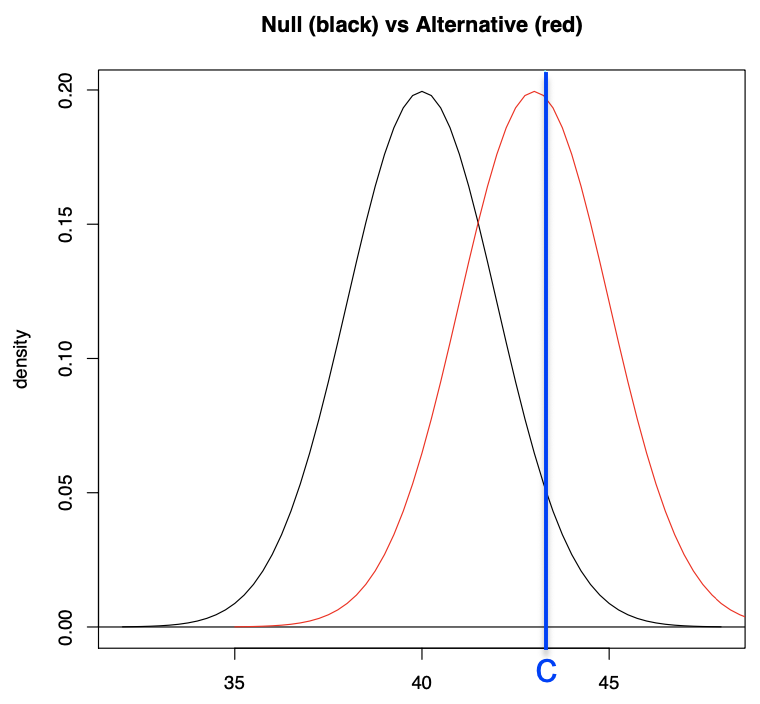
\includegraphics[width=0.65\linewidth]{st2132-hypothesis-testing-c.png} 
  \end{tightcenter}

  \subsubsection{Two-tailed test}

  $\seq x$ are from iid $N(\mu, \sigma^2)$ RVs, $\sigma$ known

  \begin{tightcenter}
    $H_0: \mu = \mu_0$, $\quad H_1 : \mu = \mu_1 \neq \mu_0$
  \end{tightcenter}

  \begin{itemize}
    \item reject $H_0$ if $\vert \xbar - \mu_0 \vert > c$, \ for some  $c>0$
      \begin{itemize}
        \item \textbf{rejection region:} $\; (-\infty,\; \mu_0 - c)$ and $(\mu_0 + c, \infty)$
      \end{itemize}
    \item $\alpha = P_{H_0} ( \vert \Xbar - \mu_0 \vert > c ) = \Pr \left( \vert Z \vert > \frac{c}{\sigma/\sqrt n} \right)$
      $\quad = 2\Pr \left( Z > \frac{c}{\sigma/\sqrt n} \right)$
    \item $c = z_{\frac{\alpha}{2}} \frac{\sigma}{\sqrt n}$
      \begin{itemize}
        \item \textbf{rejection region:} $\scriptstyle (-\infty,\; \mu_0 - z_{\frac{\alpha}{2}}\frac{\sigma}{\sqrt n})$ $\land$ $\scriptstyle (\mu_0 + z_{\frac{\alpha}{2}}\frac{\sigma}{\sqrt n}, \infty)$
      \end{itemize}
  \end{itemize}

  \subsection{Composite hypothesis}

  \begin{itemize}
    \item \definition[hypothesis]{simple} specify a single value 
      ($H_0 : \mu = \mu_0, H_1 : \mu = \mu_1$)
    \item \definition[hypothesis]{composite} range of values 
      \begin{itemize}
        \item one-tailed test: $\; H_0 : \mu = \mu_0, \; H_1 : \mu > \mu_0$
          \begin{itemize}
            \item rejection region: $(\mu_0 + z_{\alpha}\frac{\sigma}{\sqrt n}, \; \infty)$ 
              \\* $\Rightarrow$ no change since it doesn't involve $\mu_1$
          \end{itemize}
        \item two-tailed test: $\; H_0 : \mu = \mu_0, \; H_1 : \mu \neq \mu_0$
          \begin{itemize}
            \item rejection region: 
              \\* $\scriptstyle (-\infty,\; \mu_0 - z_{\frac{\alpha}{2}}\frac{\sigma}{\sqrt n})$ $\land$ $\scriptstyle (\mu_0 + z_{\frac{\alpha}{2}}\frac{\sigma}{\sqrt n}, \infty)$
              \\* $\Rightarrow$ no change since it doesn't involve $\mu_1$
            \item if $\xbar$ falls \textit{outside} the rejection region, i.e.
              \\* $\mu_0 - z_{\frac{\alpha}{2}}\frac{\sigma}{\sqrt n} \leq \xbar \leq \mu_0 + z_{\frac{\alpha}{2}}\frac{\sigma}{\sqrt n}$
              \begin{itemize}
                \item then $H_0$ is NOT rejected at level $\alpha$
                \item $\mu_0$ lies in the $(1-\alpha)$-CI for $\mu$
              \end{itemize}
          \end{itemize}
        \item as $n \to \infty$, power  $\to 1$
      \end{itemize}
  \end{itemize}

  \subsection{Hypothesis testing and CI}

  \begin{tightcenter}
    the $(1-\alpha)$-CI for $\mu$, 
    $\left( \xbar - z_{\frac{\alpha}{2}} \frac{\hat\sigma}{\sqrt n}, \xbar + z_{\frac{\alpha}{2}} \frac{\hat\sigma}{\sqrt n} \right)$

    consists of the values $\mu_0$ for which the test

    $H_0 : \mu = \mu_0, \; H_1 : \mu \neq \mu_0$
    is not rejected at level $\alpha$.
  \end{tightcenter}

  \subsection{$P$-value}

  \begin{itemize}
    \item \definition{$P$-value} the probability under $H_0$ that the random test statistic is more extreme than the observed test statistic
      \begin{itemize}
        \item small $p$-value = more "extreme" (more doubt)
      \end{itemize}
    \item reject $H_0$ at level $\alpha \iff P<\alpha$
    \item generally, $P$-value for two-tailed test is double that of one-tailed test
  \end{itemize}

  \subsubsection{formulae for $P$-value}

  $H_1 : \mu > \mu_0$ 

  $\qquad$ $P = P_{H_0} (\Xbar > \xbar) = \Pr \left( Z > \frac{\xbar - \mu_0}{\sigma / \sqrt n} \right)$

  $H_1 : \mu < \mu_0$ 

  $\qquad$ $P = P_{H_0} (\Xbar < \xbar) = \Pr \left( Z < \frac{\xbar - \mu_0}{\sigma / \sqrt n} \right)$

  $H_1 : \mu \neq \mu_0$

  $\quad$ $P = P_{H_0} (| \Xbar-\mu_0 | > | \xbar-\mu_0 |) = \Pr \left( |Z| > \frac{|\xbar - \mu_0|}{\sigma / \sqrt n} \right)$

  \section{10. GOODNESS-OF-FIT}

  \begin{itemize}
    \item \definition[(LR) test]{likelihood ratio} based on the ratio of likelihoods
      \begin{itemize}
        \item $P$-value can be approximated using $\chi^2$ distribution for a large sample size
      \end{itemize}
  \end{itemize}

  \subsection{multinomial}

  let $X \sim Trinomial(n, \mathbf{p})$. 
  by HWE, $\mathbf{p}$ is a function of $\theta$ as follows: $p_1 = (1-\theta)^2, \;p_2 = 2\theta(1-\theta), \; p_3 = \theta^2$

  let $L_1$ and $L_0$ be the maximum likelihood value for the general model ($Trinomial(n, \mathbf{p})$) and the HWE.

  \begin{itemize}
    \item $L_1 \geq L_0$ $\quad$ ($L_0$ is the maximum over a subset of $L_1$)
      \begin{itemize}
        \item general trinomial
          \begin{itemize}
            \item likelihood, $L(\mathbf{p}) = p_1^{x_1}p_2^{x_2}p_3^{x_3}$
            \item ML estimate of $\mathbf{p}$ is $\frac{x}{n}$
            \item $\log L_1 = x_1 \log (\frac{x_1}{n}) + x_2 \log (\frac{x_2}{n}) + x_3 \log (\frac{x_3}{n})$
          \end{itemize}
        \item HWE: 
          \begin{itemize}
            \item likelihood, $L(\theta) = p_1(\theta)^{x_1} p_2(\theta)^{x_2} p_3(\theta)^{x_3}$
            \item ML estimate of $\theta$ is $\frac{x_2 + 2x_3}{2n}$
          \end{itemize}
      \end{itemize}
    \item larger $L_1 / L_0 \Rightarrow$ poorer fit for HWE
  \end{itemize}

  \subsubsection{LR test}

  \begin{itemize}
    \item null hypothesis: HWE holds
      $\quad H_0: p_1 = (1-\theta)^2, \; p_2 = 2\theta(1-\theta), \; p_3 = \theta^2$
    \item LR test statistic: 
      $\quad 2 \log \left( \frac{L_1}{L_0} \right) = 2( \log L_1 - \log L_0 )$
    \item degree of freedom $=$ difference in the number of parameters between the models
      \begin{itemize}
        \item general model has 2 params, HWE has 1 param
      \end{itemize}
    \item $P$-value  $= \Pr \left(\chi_1^2 > 2\log(\frac{L_1}{L_0})\right)$
  \end{itemize}

  \subsubsection{Nested models}

  \begin{tightcenter}
    the set of all $Trinomial(n, \mathbf{p})$ distributions \\* can be represented by 
    $\Omega_1 = \left\{ (p_1, p_2, p_3) : p_i > 0, \; \sum^3_{i=1}p_i = 1 \right\}$ 

    which has dimension 2 $\quad$ ($\dim\Omega_1 = 2$)
  \end{tightcenter}

  \begin{itemize}
    \item by HWE, $\mathbf{p}$ is in the subset 
      $\quad \Omega_0 = \left\{ ( (1-\theta)^2, 2\theta(1-\theta), \theta^2 ) : 0 < \theta < 1 \right\}$
      $\quad$ ($\dim\Omega_0 = 1$)
    \item $\Omega_0$ is \ildefinition{nested} in $\Omega_1$
    \item measure goodness-of-fit of HWE by testing $H_0 : \mathbf{p} \in \Omega_0$
  \end{itemize}

  \subsection{General Multinomial LR test}

  let $(\seq[k]{X}) \sim Multinomial(n, \mathbf{p})$. 
  then $\mathbf{p} \in \Omega_1$, the set of all positive probability vectors of length $k$.

  \smallskip
  to test if $\mathbf{p}$ is in a subspace
  $\quad\Omega_0 = \left\{ (p_1(\theta), \dots, p_k(\theta)) : \theta \in \Theta \subset \mathbb{R}^h \right\}$ 

  with $\dim\Omega_0 < \dim\Omega_1 = k-1$

  \begin{tightcenter}

    let $L_j$ be the maximum likelihood value under $\Omega_j$. 

    To test $H_0 : \mathbf{p} \in \Omega_0$, we use the \ildefinition{LR statistic}, $G = 2\log(\frac{L_1}{L_0})$
  \end{tightcenter}

  \begin{itemize}
    \item for $\Omega_1$: $\log L_1 = \sum^k_{i=1} X_i \log (\frac{X_i}{n})$
    \item for $\Omega_0$: $\log L_0 = \sum^k_{i=1} X_i \log p_i(\hat\theta)$
  \end{itemize}

  \begin{tightcenter}
    $G = 2\sum^k_{i=1} X_i \log \left( \frac{X_i}{np_i(\hat\theta)} \right)$
  \end{tightcenter}

  given data $(\seq x)$, let $g$ be a realisation of $G$. 
  $P$-value $P_{H_0} (G > g)$ is approximately $\Pr (\chi^2_{k-1-\dim\Omega_0} > g)$ for large $n$.

  \begin{itemize}
    \item to compute $g$, replace
      \begin{itemize}
        \item $X_i$ with \textit{observed count} $x_i$
        \item $np_i(\hat\theta)$ with \textit{expected count}, calculated using ML estimate of  $\theta$
      \end{itemize}
  \end{itemize}

  \subsection{Test of independence}

  for a population with attributes $q$ and $r$, 
  let $p_{ij}$ be the population proportion of people with $q=q_i$ and $r=r_j$.
  for any $i, j$, $p_{ij} = q_i \times r_j$.

  \begin{itemize}
    \item let $(X_{ij}, 1 \leq i \leq I, 1 \leq j \leq J) \sim Multinomial(n, \mathbf{p})$.
      $\mathbf{p} \in \Omega_1$, where $\dim \Omega_1 = IJ - 1 = k-1$.
    \item $H_0 : $ the two categories $q,r$ are independent
      \begin{itemize}
        \item if $q,r$ are independent, then $\exists $ positive numbers $\sum^I_{i=1}q_i = \sum^J_{j=1}r_j = 1$
          such that $p_{ij} = q_i \times r_j$, $\; 1 \leq i \leq I, 1 \leq j \leq J$
      \end{itemize}
    \item $\dim\Omega_0 = (I-1) + (J-1) = I+J-2$
    \item $\dim\Omega_1 - \dim\Omega_0 = (I-1)(J-1)$
    \item under independence ($H_0$), for large  $n$, approximately $G \sim \chi^2_{(I-1)(J-1)}$
  \end{itemize}

  \subsubsection{G statistic}

  for any $i$, let $X_{i+} = \sum^J_{j=1}X_{ij}$. 

  for any $j$, let $X_{+j} = \sum^I_{i=1}X_{ij}$.

  \begin{itemize}
    \item $\Omega_1$ : $\log L_1 = \sum_{ij} X_{ij} \log \left( \frac{X_{ij}}{n} \right)$
    \item $\Omega_0$ : $\log L_0 = \sum_i X_{i+} \log \left( \frac{X_{i+}}{n} \right) + \sum_{+j} X_{+j} \log \left( \frac{X_{+j}}{n} \right)$
    \item $G = 2(\log L_1 - \log L_0) = 2\sum_{ij} X_{ij} \log \left( \frac{X_{ij}}{X_{i+} X_{+j}/n} \right)$ 
    \item the data $x_{ij}$ are the \textit{observed counts}
    \item the data $x_{i+} x_{+j}/n$ are the \textit{expected counts}
    \item $P$-value $= \Pr\left(\chi^2_{(I-1)(J-1)} > g\right)$
  \end{itemize}

  \subsection{General LR test}

  we have $n$ iid RVs with density defined by $\theta \in \Omega_1$ of dimension $k_1$;
  nested in $\Omega_1$ is a smaller model $\Omega_0$ of dimension $k_0$.

  \begin{tightcenter}
    $H_0 : \theta \in \Omega_0 \qquad H_1 : \theta \in \Omega_1 \backslash \Omega_0$

    to test $H_0 : \theta \in \Omega_0$, we use LR statistic 

    $G = 2\log \left(\frac{L_1}{L_0}\right)$

    where $L_j$ is the maximum likelihood value over $\Omega_j$.
  \end{tightcenter}

  for large $n$, the $P$-value can be approximately computed, because:

  \begin{tightcenter}
    if $\theta \in \Omega_0$, as $n \to \infty$, 

    the distribution of $G$ converges to $\chi^2_{k_1-k_0}$
  \end{tightcenter}

  \subsubsection{Normal LR test}

  $\seq x$ are form iid $N(\mu, \sigma^2)$ RVs.
  to test $H_0 : \mu = 0$:

  $ \begin{array}{c|c|c|c|c}
    \sigma & \Omega_1 & k_1 & \Omega_0 & k_0 \\\hline
    \text{known} & \mathbb{R} & 1 & \{0\} & 0 \\
    \text{unknown} & \mathbb{R}\times \mathbb{R}_+ & 2 & \{0\} \times \mathbb{R}_+ & 1
  \end{array} $

  under $H_0$, for large $n$, approximately $G \sim \chi^2_1$

  \begin{itemize}
    \item \textbf{case 1}: $\sigma$ known
      \begin{itemize}
        \item $\Omega_1 : \log L_1 = -\frac{n\hat\sigma^2}{2\sigma^2}$
        \item $\Omega_0 : \log L_0 = -\frac{n\hat\mu^2}{2\sigma^2}$ 
        \item $G = 2(\log L_1 - \log L_0) = \frac{n\Xbar^2}{\sigma^2}$
          \begin{itemize}
            \item if $H_0$ holds ($\mu = 0$), then $\Xbar \sim N(0, \frac{\sigma^2}{n})$. 
              for any $n$, $G \sim \chi^2_1$ exactly.
          \end{itemize}
      \end{itemize}

    \item \textbf{case 2}: $\sigma$ unknown
      \begin{itemize}
        \item $\Omega_1 : \log L_1 = -\frac{n}{2} \log \hat\sigma^2 - \frac{n}{2}$
        \item $\Omega_0 : \log L_0 = -\frac{n}{2} \log \hat\mu_2 - \frac{n}{2}$
        \item $G = 2(\log L_1 - \log L_0) = n\log ( \frac{\hat\mu_2}{\hat\sigma^2} )$
        \item if $H_0$ holds ($\mu = 0$), for large $n$, $G \sim \chi^2_1$ approximately
      \end{itemize}
  \end{itemize}

  \subsection{Summary}

  \begin{itemize}
    \item LR test applies when the investigator wants to know the goodness-of-fit of a model relative to a larger model, of dimensions $k_0 < k_1$.
    \item test statistic, $G = 2\log \left( \frac{L_1}{L_0} \right)$
      \begin{itemize}
        \item $L_0, L_1$ are the maximum likelihood value under the small and large models
      \end{itemize}
    \item if $n$ is large, the $P$-value $\Pr (G > g)$ (computed provided $H_0$ is true) can be approximated by a $\chi^2_{k_1-k_0}$ distribution
  \end{itemize}




\end{multicols*}

\end{document}
